\begin{figure*}[!t]
    \centering
    {
        \newlength\mytmplennvs
        \setlength\mytmplennvs{.11\linewidth}
        \setlength\tabcolsep{0pt}
        \begin{tabular}{ccccccccc}
            \hspace{-4mm}
            \redbox{./img/nvs/materials/nerfactor}{(0.8,0.1)}{(1.2,0.5)}{\mytmplennvs}&
            \redbox{./img/nvs/materials/tensoir}{(0.8,0.1)}{(1.2,0.5)}{\mytmplennvs}&
            \redbox{./img/nvs/materials/ndr}{(0.8,0.1)}{(1.2,0.5)}{\mytmplennvs}&
            \redbox{./img/nvs/materials/nero}{(0.8,0.1)}{(1.2,0.5)}{\mytmplennvs}&
            \redbox{./img/nvs/materials/gs}{(0.8,0.1)}{(1.2,0.5)}{\mytmplennvs}&
            \redbox{./img/nvs/materials/rgs}{(0.8,0.1)}{(1.2,0.5)}{\mytmplennvs}&
            \redbox{./img/nvs/materials/gshader}{(0.8,0.1)}{(1.2,0.5)}{\mytmplennvs}&
            \redbox{./img/nvs/materials/ours}{(0.8,0.1)}{(1.2,0.5)}{\mytmplennvs}&
            \redbox{./img/nvs/materials/gt}{(0.8,0.1)}{(1.2,0.5)}{\mytmplennvs}
            \\
            \hspace{-4mm}
            \redbox{./img/nvs/mic/nerfactor}{(0.8,1.6)}{(1.2,2)}{\mytmplennvs}&
            \redbox{./img/nvs/mic/tensoir}{(0.8,1.6)}{(1.2,2)}{\mytmplennvs}&
            \redbox{./img/nvs/mic/ndr}{(0.8,1.6)}{(1.2,2)}{\mytmplennvs}&
            \redbox{./img/nvs/mic/nero}{(0.8,1.6)}{(1.2,2)}{\mytmplennvs}&
            \redbox{./img/nvs/mic/gs}{(0.8,1.6)}{(1.2,2)}{\mytmplennvs}&
            \redbox{./img/nvs/mic/rgs}{(0.8,1.6)}{(1.2,2)}{\mytmplennvs}&
            \redbox{./img/nvs/mic/gshader}{(0.8,1.6)}{(1.2,2)}{\mytmplennvs}&
            \redbox{./img/nvs/mic/ours}{(0.8,1.6)}{(1.2,2)}{\mytmplennvs}&
            \redbox{./img/nvs/mic/gt}{(0.8,1.6)}{(1.2,2)}{\mytmplennvs}
            \\
            \hspace{-4mm}
            \redbox{./img/nvs/teapot/nerfactor}{(1,0.5)}{(1.5,1)}{\mytmplennvs}&
            \redbox{./img/nvs/teapot/tensoir}{(1,0.5)}{(1.5,1)}{\mytmplennvs}&
            \redbox{./img/nvs/teapot/ndr}{(1,0.5)}{(1.5,1)}{\mytmplennvs}&
            \redbox{./img/nvs/teapot/nero}{(1,0.5)}{(1.5,1)}{\mytmplennvs}&
            \redbox{./img/nvs/teapot/gs}{(1,0.5)}{(1.5,1)}{\mytmplennvs}&
            \redbox{./img/nvs/teapot/rgs}{(1,0.5)}{(1.5,1)}{\mytmplennvs}&
            \redbox{./img/nvs/teapot/gshader}{(1,0.5)}{(1.5,1)}{\mytmplennvs}&
            \redbox{./img/nvs/teapot/ours}{(1,0.5)}{(1.5,1)}{\mytmplennvs}&
            \redbox{./img/nvs/teapot/gt}{(1,0.5)}{(1.5,1)}{\mytmplennvs}
            \\
             \hspace{-4mm}
            \redbox{./img/nvs/coffee/nerfactor}{(0.7,0.4)}{(1.5,1.2)}{\mytmplennvs}&
            \redbox{./img/nvs/coffee/tensoir}{(0.7,0.4)}{(1.5,1.2)}{\mytmplennvs}&
            \redbox{./img/nvs/coffee/ndr}{(0.7,0.4)}{(1.5,1.2)}{\mytmplennvs}&
            \redbox{./img/nvs/coffee/nero}{(0.7,0.4)}{(1.5,1.2)}{\mytmplennvs}&
            \redbox{./img/nvs/coffee/gs}{(0.7,0.4)}{(1.5,1.2)}{\mytmplennvs}&
            \redbox{./img/nvs/coffee/rgs}{(0.7,0.4)}{(1.5,1.2)}{\mytmplennvs}&
            \redbox{./img/nvs/coffee/gshader}{(0.7,0.4)}{(1.5,1.2)}{\mytmplennvs}&
            \redbox{./img/nvs/coffee/ours}{(0.7,0.4)}{(1.5,1.2)}{\mytmplennvs}&
            \redbox{./img/nvs/coffee/gt}{(0.7,0.4)}{(1.5,1.2)}{\mytmplennvs}
            \\
            \hspace{-4mm}
            \redbox{./img/nvs/baking_scene001/nerfactor}{(0.5,2)}{(1.6,1.2)}{\mytmplennvs}&
            \redbox{./img/nvs/baking_scene001/tensoir}{(0.5,2)}{(1.6,1.2)}{\mytmplennvs}&
            \redbox{./img/nvs/baking_scene001/ndr}{(0.5,2)}{(1.6,1.2)}{\mytmplennvs}&
            \redbox{./img/nvs/baking_scene001/nero}{(0.5,2)}{(1.6,1.2)}{\mytmplennvs}&
            \redbox{./img/nvs/baking_scene001/gs}{(0.5,2)}{(1.6,1.2)}{\mytmplennvs}&
            \redbox{./img/nvs/baking_scene001/rgs}{(0.5,2)}{(1.6,1.2)}{\mytmplennvs}&
            \redbox{./img/nvs/baking_scene001/gshader}{(0.5,2)}{(1.6,1.2)}{\mytmplennvs}&
            \redbox{./img/nvs/baking_scene001/ours}{(0.5,2)}{(1.6,1.2)}{\mytmplennvs}&
            \redbox{./img/nvs/baking_scene001/gt}{(0.5,2)}{(1.6,1.2)}{\mytmplennvs}
            \\
            \hspace{-4mm}
            \redbox{./img/nvs/car_scene002/nerfactor}{(0.85,0.2)}{(1.9,1)}{\mytmplennvs}&
            \redbox{./img/nvs/car_scene002/tensoir}{(0.85,0.2)}{(1.9,1)}{\mytmplennvs}&
            \redbox{./img/nvs/car_scene002/ndr}{(0.85,0.2)}{(1.9,1)}{\mytmplennvs}&
            \redbox{./img/nvs/car_scene002/nero}{(0.85,0.2)}{(1.9,1)}{\mytmplennvs}&
            \redbox{./img/nvs/car_scene002/gs}{(0.85,0.2)}{(1.9,1)}{\mytmplennvs}&
            \redbox{./img/nvs/car_scene002/rgs}{(0.85,0.2)}{(1.9,1)}{\mytmplennvs}&
            \redbox{./img/nvs/car_scene002/gshader}{(0.85,0.2)}{(1.9,1)}{\mytmplennvs}&
            \redbox{./img/nvs/car_scene002/ours}{(0.85,0.2)}{(1.9,1)}{\mytmplennvs}&
            \redbox{./img/nvs/car_scene002/gt}{(0.85,0.2)}{(1.9,1)}{\mytmplennvs}
            \\
            \hspace{-4mm}
            NeRFactor&
            \wttp{TensoIR}&
            NDR&
            NeRO&
            GS&
            RGS&
            GShader&
            Ours&
            GT
        \end{tabular}
    }
    \caption{Novel view synthesis comparisons with NeRFactor~\cite{NeRFactor}, \wttp{TensoIR~\cite{TensoIR}}, NDR~\cite{NvDiffRec}, NeRO~\cite{NeRO}, Gaussian Splatting (GS)~\cite{GS}, RelightableGaussian (RGS)~\cite{RelightableGaussian}, and GaussianShader (GShader)~\cite{GaussianShader}. 
    The bottom two rows are from the real Stanford ORB dataset~\cite{Stanford-ORB}.
    }
    \label{fig:nvs}
\end{figure*}

\begin{table*}[!t]
	\caption{
		\wttp{Quantitative comparison of novel view synthesis results using SSIM, PSNR and LPIPS metrics on NeRF Synthetic, Shiny Blender and Stanford ORB datasets.}
	}
		\centering
				\begin{tabular*}{\linewidth}{@{\extracolsep{\fill}} cccccccccc }

\hline
				    \multirow{2}[2]{*}{Methods} &                           \multicolumn{3}{c}{\tabincell{c}{NeRF Synthetic}}                            &                            \multicolumn{3}{c}{\tabincell{c}{Shiny Blender}}                            &  \multicolumn{3}{c}{\tabincell{c}{Stanford ORB}} \\ 
                    \cmidrule{2-10}             & \tabincell{c}{PSNR $^\uparrow$} & \tabincell{c}{SSIM $^\uparrow$} & \tabincell{c}{LPIPS $^\downarrow$} & \tabincell{c}{PSNR $^\uparrow$} & \tabincell{c}{SSIM $^\uparrow$} & \tabincell{c}{LPIPS $^\downarrow$} & \tabincell{c}{PSNR $^\uparrow$} & \tabincell{c}{SSIM $^\uparrow$} & \tabincell{c}{LPIPS $^\downarrow$}  \\ \hline

				    NeRFactor                   & 27.86                           & 0.924                           & 0.044                              & 27.04                           & 0.913                           & 0.123                              & 30.01 & 0.934 & 0.079\\
				    TensoIR                     & 29.52                           & \tbc{0.944}                     & 0.050                              & 28.01                           & 0.905                           & 0.131                              & 34.16 & 0.980 & 0.020\\
				    NDR                         & 29.05                           & 0.939                           & 0.081                              & 28.11                           & 0.935                           & 0.076                              & 32.84 & 0.985 & 0.014\\
				    NeRO                        & 29.03                           & 0.942                           & 0.051                              & \sbc{30.96}                     & \sbc{0.953}                     & \sbc{0.045}                        & 29.25 & 0.970 & 0.019\\
				    GS                          & \bc{33.30}                      & \sbc{0.969}                     & \bc{0.030}                         & 30.35                           & 0.944                           & 0.088                              & \tbc{35.77} & \tbc{0.991} & \tbc{0.007}\\
				    RGS                         & 29.25                           & 0.941                           & \tbc{0.042}                        & 28.69                           & 0.930                           & 0.081                              & \sbc{36.65} & \sbc{0.992} & \bc{0.006}\\
				    GShader                     & \tbc{30.84}                     & 0.933                           & 0.067                              & \tbc{30.72}                     & \tbc{0.951}                     & \tbc{0.069}                        & 35.43 & 0.990 & 0.008\\ \hline
				    Ours                        & \sbc{32.29}                     & \bc{0.971}                      & \sbc{0.039}                        & \bc{32.61}                      & \bc{0.968}                      & \bc{0.041}                         & \bc{37.93} & \bc{0.995} & \bc{0.006}\\ %
\hline
				\end{tabular*}
	\label{tab:nvs}
\end{table*}




\section{Results and Evaluations}
\subsection{Datasets and Metrics}
\wttp{We conduct qualitative and quantitative experiments on two synthetic datasets, NeRF Synthetic~\cite{NeRF} and Shiny Blender~\cite{RefNeRF} and one real dataset, the Stanford ORB dataset ~\cite{Stanford-ORB}.
For all datasets, we evaluate \name and baseline methods on novel view synthesis,  decomposition and relighting tasks. 
For quantitative comparisons, we use PSNR (Peak Signal-to-Noise Ratio), SSIM (Structural Similarity)~\cite{SSIM} and LPIPS (Learned Perceptual Image Patch Similarity)~\cite{LPIPS} metrics to compare the similarity between images. 
To evaluate the quality of the estimated normals, we compare the estimated normal images with the ground truth with Mean Squared Error (MSE). 
}

\subsection{Implementation Details}
\wttp{
We train the decoupled Gaussian splatting representation on a single 3090 GPU with 24GB memory. 
The training process takes 3-4 hours depending on the scenes' complexity and the input images' resolution. 
\name allows $\sim$30FPS novel view synthesis at $800 \times 800$ resolution on a single 3090 GPU. 
For hyperparameter settings, in Eqn.~(\ref{eqn:loss_refneus}), $\lambda_{1}$ is set to $0.1$.  
In Eqn.~(\ref{eqn:total_loss}), $\lambda_{nd}, \lambda_{L1}, \lambda_{ssim}, \lambda_{mask} ,\lambda_{TV}$ are set to $0.5, 0.8, 0.2, 0.5, 0.001$ in all our examples. 
}

\subsection{Novel View Synthesis}
We present novel view synthesis results on different cases' test splits in Fig.~\ref{fig:nvs} and compare \yl{our method} with NeRFactor~\cite{NeRFactor}, \wttp{TensoIR}~\cite{TensoIR}, NDR~\cite{NvDiffRec}, NeRO~\cite{NeRO}, Gaussian Splatting~\cite{GS}, RelightableGaussian~\cite{RelightableGaussian} and GuassianShader~\cite{GaussianShader}. 
NeRFactor models the geometry with a density function and utilizes a low-resolution environment map as its lighting representation, which leads to less convincing geometry (first row in Fig.~\ref{fig:nvs}) and blurry reconstruction results. 
\wttp{TensoIR is unable to synthesize appearance details with its smooth lighting representation approximated by Spherical Gaussian functions. }
NDR uses deformable \yl{tetrahedra} to approximate the geometry which may cause irregular geometry and noisy novel view synthesis results. 
\wt{NeRO produces blurry appearance (second and fourth rows) and may reconstruct wrong geometry (first row).}
\yl{Gaussian} Splatting models the texture and lighting with a single spherical harmonic function which may fail to generalize to novel views and produce wrong reflections (last row in Fig.~\ref{fig:nvs}). 
RelightableGaussian and GaussianShader separately model texture and lighting but learn geometry from scratch, which causes blurry reconstruction. 
As for quantitative comparisons, we compare novel view reconstruction results by different methods with the ground truth image using PSNR, SSIM and LPIPS metrics in Table~\ref{tab:nvs}. 
\wt{Our method achieves comparable results with baseline methods on the NeRF synthetic dataset and outperforms other baselines on the shiny blender dataset.}

\begin{figure*}[t!]
    \centering
    {
        \newlength\mytmplen
        \setlength\mytmplen{.11\linewidth}
        \setlength\tabcolsep{0pt}
            \setlength\tabcolsep{0pt}
            \begin{tabular*}{\textwidth}{@{\extracolsep{\fill}} ccccccccc }
                \hspace{-1mm}{\rotatebox{90}{\quad \hspace{4mm} {Normal}}}&
                \hspace{-2mm}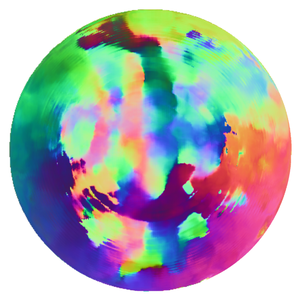
\includegraphics[width=0.12\textwidth]{./img/decom/ball/nerfactor_n}&
                \hspace{-2mm}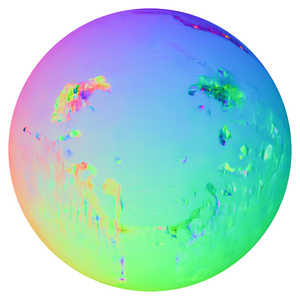
\includegraphics[width=0.12\textwidth]{./img/decom/ball/tensoir_n}&
                \hspace{-2mm}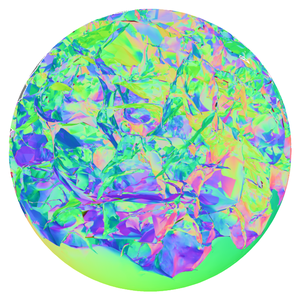
\includegraphics[width=0.12\textwidth]{./img/decom/ball/ndr_n}&
                \hspace{-2mm}
\includegraphics[width=0.12\textwidth]{./img/decom/ball/nero_n}&
                \hspace{-2mm}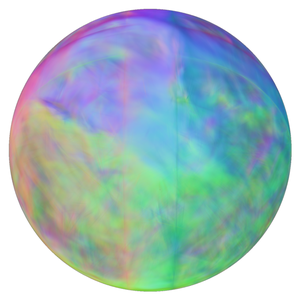
\includegraphics[width=0.12\textwidth]{./img/decom/ball/rgs_n}&
                \hspace{-2mm}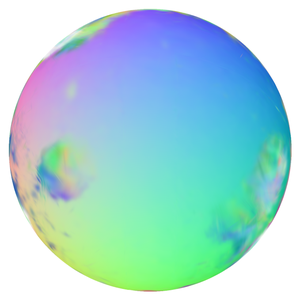
\includegraphics[width=0.12\textwidth]{./img/decom/ball/gshader_n}&
                \hspace{-2mm}
\includegraphics[width=0.12\textwidth]{./img/decom/ball/ours_n}&
                \hspace{-2mm}
\includegraphics[width=0.12\textwidth]{./img/decom/ball/gt_n}
                \\
                \hspace{-1mm}{\rotatebox{90}{\quad \hspace{4mm} {\makecell{Albedo}}}}&
                \hspace{-2mm}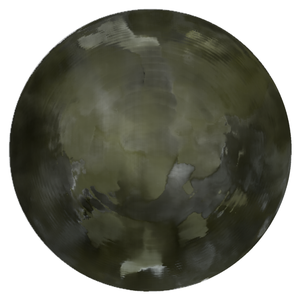
\includegraphics[width=0.12\textwidth]{./img/decom/ball/nerfactor_a}&
                \hspace{-2mm}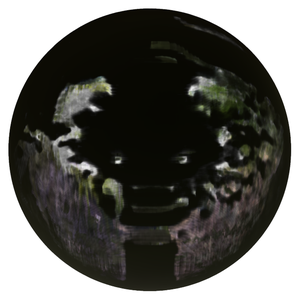
\includegraphics[width=0.12\textwidth]{./img/decom/ball/tensoir_a}&
                \hspace{-2mm}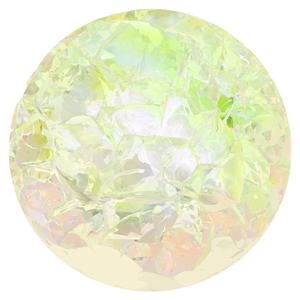
\includegraphics[width=0.12\textwidth]{./img/decom/ball/ndr_a}&
                \hspace{-2mm}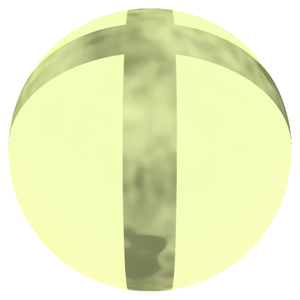
\includegraphics[width=0.12\textwidth]{./img/decom/ball/nero_a}&
                \hspace{-2mm}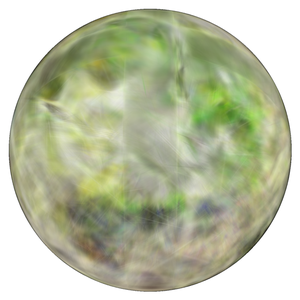
\includegraphics[width=0.12\textwidth]{./img/decom/ball/rgs_a}&
                \hspace{-2mm}
\includegraphics[width=0.12\textwidth]{./img/na}&
                \hspace{-2mm}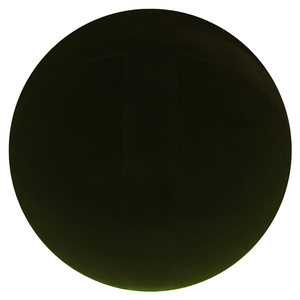
\includegraphics[width=0.12\textwidth]{./img/decom/ball/ours_a}&
                \hspace{-2mm}
\includegraphics[width=0.12\textwidth]{./img/decom/ball/gt_a}
                \vspace{-2mm}
                \\
                \vspace{-2mm}
                \hspace{-1mm}{\rotatebox{90}{\quad \hspace{4mm} {Normal}}}&
                \hspace{-2mm}
\includegraphics[width=0.12\textwidth]{./img/decom/helmet/nerfactor_n}&
                \hspace{-2mm}
\includegraphics[width=0.12\textwidth]{./img/decom/helmet/tensoir_n}&
                \hspace{-2mm}
\includegraphics[width=0.12\textwidth]{./img/decom/helmet/ndr_n}&
                \hspace{-2mm}
\includegraphics[width=0.12\textwidth]{./img/decom/helmet/nero_n}&
                \hspace{-2mm}
\includegraphics[width=0.12\textwidth]{./img/decom/helmet/rgs_n}&
                \hspace{-2mm}
\includegraphics[width=0.12\textwidth]{./img/decom/helmet/gshader_n}&
                \hspace{-2mm}
\includegraphics[width=0.12\textwidth]{./img/decom/helmet/ours_n}&
                \hspace{-2mm}
\includegraphics[width=0.12\textwidth]{./img/decom/helmet/gt_n}
                \\
                \hspace{-1mm}{\rotatebox{90}{\quad \hspace{4mm} {\makecell{Albedo}}}}&
                \hspace{-2mm}
\includegraphics[width=0.12\textwidth]{./img/decom/helmet/nerfactor_a}&
                \hspace{-2mm}
\includegraphics[width=0.12\textwidth]{./img/decom/helmet/tensoir_a}&
                \hspace{-2mm}
\includegraphics[width=0.12\textwidth]{./img/decom/helmet/ndr_a}&
                \hspace{-2mm}
\includegraphics[width=0.12\textwidth]{./img/decom/helmet/nero_a}&
                \hspace{-2mm}
\includegraphics[width=0.12\textwidth]{./img/decom/helmet/rgs_a}&
                \hspace{-2mm}
\includegraphics[width=0.12\textwidth]{./img/na}&
                \hspace{-2mm}
\includegraphics[width=0.12\textwidth]{./img/decom/helmet/ours_a}&
                \hspace{-2mm}
\includegraphics[width=0.12\textwidth]{./img/decom/helmet/gt_a}
                \\
                \hspace{-1mm}{\rotatebox{90}{\quad \hspace{0mm} {Normal}}}&
                \zoomin{./img/decom/ficus/nerfactor_n}{0.5}{0.25}{1.4}{0.5}{1.15cm}{\mytmplen}{2}{south west}&
                \zoomin{./img/decom/ficus/tensoir_n}{0.5}{0.25}{1.4}{0.5}{1.15cm}{\mytmplen}{2}{south west}&
                \zoomin{./img/decom/ficus/ndr_n}{0.5}{0.25}{1.4}{0.5}{1.15cm}{\mytmplen}{2}{south west}&
                \zoomin{./img/decom/ficus/nero_n}{0.5}{0.25}{1.4}{0.5}{1.15cm}{\mytmplen}{2}{south west}&
                \zoomin{./img/decom/ficus/rgs_n}{0.5}{0.25}{1.4}{0.5}{1.15cm}{\mytmplen}{2}{south west}&
                \zoomin{./img/decom/ficus/gshader_n}{0.5}{0.25}{1.4}{0.5}{1.15cm}{\mytmplen}{2}{south west}&
                \zoomin{./img/decom/ficus/ours_n}{0.5}{0.25}{1.4}{0.5}{1.15cm}{\mytmplen}{2}{south west}&
                \zoomin{./img/decom/ficus/gt_n}{0.5}{0.25}{1.4}{0.5}{1.15cm}{\mytmplen}{2}{south west}
                \\
                \hspace{-1mm}{\rotatebox{90}{\quad \hspace{0mm} {\makecell{Albedo}}}}&
                \zoomin{./img/decom/ficus/nerfactor_a}{0.5}{0.3}{1.4}{0.5}{1.15cm}{\mytmplen}{2}{south west}&
                \zoomin{./img/decom/ficus/tensoir_a}{0.5}{0.3}{1.4}{0.5}{1.15cm}{\mytmplen}{2}{south west}&
                \zoomin{./img/decom/ficus/ndr_a}{0.5}{0.3}{1.4}{0.5}{1.15cm}{\mytmplen}{2}{south west}&
                \zoomin{./img/decom/ficus/nero_a}{0.5}{0.3}{1.4}{0.5}{1.15cm}{\mytmplen}{2}{south west}&
                \zoomin{./img/decom/ficus/rgs_a}{0.5}{0.3}{1.4}{0.5}{1.15cm}{\mytmplen}{2}{south west}&
                \hspace{-2mm}
\includegraphics[width=0.12\textwidth]{./img/na}&
                \zoomin{./img/decom/ficus/ours_a}{0.5}{0.3}{1.4}{0.5}{1.15cm}{\mytmplen}{2}{south west}&
                \zoomin{./img/decom/ficus/gt_a}{0.5}{0.3}{1.4}{0.5}{1.15cm}{\mytmplen}{2}{south west}
                \\
                \hspace{-1mm}{\rotatebox{90}{\quad \hspace{4mm} {Normal}}}&
                \hspace{-2mm}
\includegraphics[width=0.12\textwidth]{./img/decom/ball_scene002/nerfactor_n}&
                \hspace{-2mm}
\includegraphics[width=0.12\textwidth]{./img/decom/ball_scene002/tensoir_n}&
                \hspace{-2mm}
\includegraphics[width=0.12\textwidth]{./img/decom/ball_scene002/ndr_n}&
                \hspace{-2mm}
\includegraphics[width=0.12\textwidth]{./img/decom/ball_scene002/nero_n}&
                \hspace{-2mm}
\includegraphics[width=0.12\textwidth]{./img/decom/ball_scene002/rgs_n}&
                \hspace{-2mm}
\includegraphics[width=0.12\textwidth]{./img/decom/ball_scene002/gshader_n}&
                \hspace{-2mm}
\includegraphics[width=0.12\textwidth]{./img/decom/ball_scene002/ours_n}&
                \hspace{-2mm}
\includegraphics[width=0.12\textwidth]{./img/decom/ball_scene002/gt_n}
                \\
                \hspace{-1mm}{\rotatebox{90}{\quad \hspace{4mm} {\makecell{Albedo}}}}&
                \hspace{-2mm}
\includegraphics[width=0.12\textwidth]{./img/decom/ball_scene002/nerfactor_a}&
                \hspace{-2mm}
\includegraphics[width=0.12\textwidth]{./img/decom/ball_scene002/tensoir_a}&
                \hspace{-2mm}
\includegraphics[width=0.12\textwidth]{./img/decom/ball_scene002/ndr_a}&
                \hspace{-2mm}
\includegraphics[width=0.12\textwidth]{./img/decom/ball_scene002/nero_a}&
                \hspace{-2mm}
\includegraphics[width=0.12\textwidth]{./img/decom/ball_scene002/rgs_a}&
                \hspace{-2mm}
\includegraphics[width=0.12\textwidth]{./img/na}&
                \hspace{-2mm}
\includegraphics[width=0.12\textwidth]{./img/decom/ball_scene002/ours_a}&
                \hspace{-2mm}
\includegraphics[width=0.12\textwidth]{./img/decom/ball_scene002/gt_a}
                \\
                \hspace{-1mm}{\rotatebox{90}{\quad \hspace{4mm} {Normal}}}&
                \hspace{-2mm}
\includegraphics[width=0.12\textwidth]{./img/decom/teapot_scene001/nerfactor_n}&
                \hspace{-2mm}
\includegraphics[width=0.12\textwidth]{./img/decom/teapot_scene001/tensoir_n}&
                \hspace{-2mm}
\includegraphics[width=0.12\textwidth]{./img/decom/teapot_scene001/ndr_n}&
                \hspace{-2mm}
\includegraphics[width=0.12\textwidth]{./img/decom/teapot_scene001/nero_n}&
                \hspace{-2mm}
\includegraphics[width=0.12\textwidth]{./img/decom/teapot_scene001/rgs_n}&
                \hspace{-2mm}
\includegraphics[width=0.12\textwidth]{./img/decom/teapot_scene001/gshader_n}&
                \hspace{-2mm}
\includegraphics[width=0.12\textwidth]{./img/decom/teapot_scene001/ours_n}&
                \hspace{-2mm}
\includegraphics[width=0.12\textwidth]{./img/decom/teapot_scene001/gt_n}
                \vspace{-4mm}
                \\
                \hspace{-1mm}{\rotatebox{90}{\quad \hspace{4mm} {\makecell{Albedo}}}}&
                \hspace{-2mm}
\includegraphics[width=0.12\textwidth]{./img/decom/teapot_scene001/nerfactor_a}&
                \hspace{-2mm}
\includegraphics[width=0.12\textwidth]{./img/decom/teapot_scene001/tensoir_a}&
                \hspace{-2mm}
\includegraphics[width=0.12\textwidth]{./img/decom/teapot_scene001/ndr_a}&
                \hspace{-2mm}
\includegraphics[width=0.12\textwidth]{./img/decom/teapot_scene001/nero_a}&
                \hspace{-2mm}
\includegraphics[width=0.12\textwidth]{./img/decom/teapot_scene001/rgs_a}&
                \hspace{-2mm}
\includegraphics[width=0.12\textwidth]{./img/na}&
                \hspace{-2mm}
\includegraphics[width=0.12\textwidth]{./img/decom/teapot_scene001/ours_a}&
                \hspace{-2mm}
\includegraphics[width=0.12\textwidth]{./img/decom/teapot_scene001/gt_a}
                \\
                &
                \makecell{NeRFactor}&
                \makecell{\wttp{TensoIR}}&
                \makecell{NDR}&
                \makecell{NeRO}&
                \makecell{RGS}&
                \makecell{GShader}&
                \makecell{Ours}&
                \makecell{GT}
            \end{tabular*}
    }
    \caption{
        Decomposed \yl{result} comparisons with NeRFactor~\cite{NeRFactor}, \wttp{TensoIR}~\cite{TensoIR}, NDR~\cite{NvDiffRec}, NeRO~\cite{NeRO}, RelightableGaussian (RGS)~\cite{RelightableGaussian}, and GaussianShader (GShader)~\cite{GaussianShader}. 
        In every two rows, we show decomposed normal and diffuse albedo components by different methods and compare \yl{them} with the ground truth. 
        Note that GaussianShader only decomposes diffuse color instead of diffuse albedo so its diffuse albedo results are unavailable. 
    }
    \label{fig:decom}
\end{figure*}

\begin{table*}[t!]
    \caption{
        Quantitative comparison of decomposed diffuse albedos and normals by different methods. 
        Diffuse albedo is evaluated with PSNR, SSIM and LPIPS metrics while estimated normals are evaluated with MSE. 
        Note that GaussianShader (GShader)~\cite{GaussianShader} only decomposes diffuse color instead of diffuse albedo so its albedo results are unavailable.
    }
                \setlength\tabcolsep{0pt}
                \begin{tabular*}{\linewidth}{@{\extracolsep{\fill}} ccccccccccccc }
\hline
                    \multirow{2}[2]{*}{Methods} &                                                         \multicolumn{4}{c}{\tabincell{c}{NeRF Synthetic}}                                                         &                                                         \multicolumn{4}{c}{\tabincell{c}{Shiny Blender}}                                                          &                                                          \multicolumn{4}{c}{\tabincell{c}{Stanford ORB}}                                                          \\ \cmidrule{2-13}
                                                & \tabincell{c}{\small PSNR$^\uparrow$} & \tabincell{c}{\small SSIM$^\uparrow$} & \tabincell{c}{\small LPIPS$^\downarrow$} & \tabincell{c}{\small MSE$^\downarrow$} & \tabincell{c}{\small PSNR$^\uparrow$} & \tabincell{c}{\small SSIM$^\uparrow$} & \tabincell{c}{\small LPIPS$^\downarrow$} & \tabincell{c}{\small MSE$^\downarrow$} & \tabincell{c}{\small PSNR$^\uparrow$} & \tabincell{c}{\small SSIM$^\uparrow$} & \tabincell{c}{\small LPIPS$^\downarrow$} & \tabincell{c}{\small MSE$^\downarrow$} \\ \hline
                    NeRFactor                   & 19.01                                 & \sbc{0.871}                           & \bc{0.086}                               & 0.098                                  & 18.28                                 & 0.854                                 & \bc{0.106}                               & 0.132                                  & 28.62                                 & 0.958                                 & 0.046                                    & 0.067                                  \\
                    TensoIR                     & \bc{20.29}                            & \sbc{0.871}                           & \sbc{0.103}                              & \sbc{0.056}                            & \sbc{20.43}                           & \sbc{0.879}                           & 0.194                                    & 0.068                                  & 29.11                                 & 0.969                                 & 0.026                                    & \sbc{0.029}                            \\
                    NDR                         & 18.34                                 & 0.859                                 & 0.116                                    & \tbc{0.064}                            & \tbc{19.66}                           & 0.865                                 & 0.192                                    & \tbc{0.058}                            & \sbc{30.67}                           & \tbc{0.971}                           & \sbc{0.023}                              & 0.043                            \\
                    NeRO                        & \sbc{19.69}                           & 0.866                                 & 0.137                                    & 0.135                                  & 18.31                                 & \tbc{0.867}                           & \sbc{0.187}                              & \bc{0.037}                             & 24.70                                 & 0.948                                 & 0.045                                    & 0.144                                  \\
                    RGS                         & 18.13                                 & 0.862                                 & 0.115                                    & 0.072                                  & 18.10                                 & 0.847                                 & 0.198                                    & 0.065                                  & \tbc{29.33}                           & \bc{0.979}                            & \tbc{0.025}                              & 0.049                                  \\
                    GShader                     & -                                     & -                                     & -                                        & 0.115                                  & -                                     & -                                     & -                                        & 0.093                                  & -                                     & -                                     & -                                        & \tbc{0.037}                            \\ \hline
                    w/o NFD                     & 16.25                                 & 0.821                                 & 0.138                                    & 0.143                                  & 16.58                                 & 0.839                                 & 0.189                                    & 0.102                                  & 29.04                                 & 0.964                                 & 0.039                                    & 0.081                                  \\
                    Ours                        & \tbc{19.14}                           & \bc{0.878}                            & \tbc{0.109}                              & \bc{0.053}                             & \bc{20.65}                            & \bc{0.883}                            & \tbc{0.188}                              & \bc{0.037}                             & \bc{31.99}                            & \sbc{0.977}                           & \bc{0.021}                               & \bc{0.024}                             \\ \hline
                \end{tabular*}
    \label{tab:decom}
\end{table*}



\begin{figure*}[!t]
    \centering
    {   
        \newlength\mytmplenrelight
        \setlength\mytmplenrelight{.11\linewidth}
        \setlength\tabcolsep{0pt}
        \begin{tabular}{ccccccccc}
            {
\includegraphics[width=0.11\linewidth]{./img/relight/toaster/courtyard/input}}&
            {
\includegraphics[width=0.11\linewidth]{./img/relight/toaster/courtyard/nerfactor}}&
            {
\includegraphics[width=0.11\linewidth]{./img/relight/toaster/courtyard/tensoir}}&
            {
\includegraphics[width=0.11\linewidth]{./img/relight/toaster/courtyard/ndr}}&
            {
\includegraphics[width=0.11\linewidth]{./img/relight/toaster/courtyard/nero}}&
            {
\includegraphics[width=0.11\linewidth]{./img/relight/toaster/courtyard/rgs}}&
            {
\includegraphics[width=0.11\linewidth]{./img/relight/toaster/courtyard/gshader}}&
            {
\includegraphics[width=0.11\linewidth]{./img/relight/toaster/courtyard/ours}}&
            {
\includegraphics[width=0.11\linewidth]{./img/relight/toaster/courtyard/gt}}
            \\
            {
\includegraphics[width=0.11\linewidth]{./img/relight/toaster/night/input}}&
            {
\includegraphics[width=0.11\linewidth]{./img/relight/toaster/night/nerfactor}}&
            {
\includegraphics[width=0.11\linewidth]{./img/relight/toaster/night/tensoir}}&
            {
\includegraphics[width=0.11\linewidth]{./img/relight/toaster/night/ndr}}&
            {
\includegraphics[width=0.11\linewidth]{./img/relight/toaster/night/nero}}&
            {
\includegraphics[width=0.11\linewidth]{./img/relight/toaster/night/rgs}}&
            {
\includegraphics[width=0.11\linewidth]{./img/relight/toaster/night/gshader}}&
            {
\includegraphics[width=0.11\linewidth]{./img/relight/toaster/night/ours}}&
            {
\includegraphics[width=0.11\linewidth]{./img/relight/toaster/night/gt}}
            \\
            {
\includegraphics[width=0.11\linewidth]{./img/relight/ball/courtyard/input}}&
            {
\includegraphics[width=0.11\linewidth]{./img/relight/ball/courtyard/nerfactor}}&
            {
\includegraphics[width=0.11\linewidth]{./img/relight/ball/courtyard/tensoir}}&
            {
\includegraphics[width=0.11\linewidth]{./img/relight/ball/courtyard/ndr}}&
            {
\includegraphics[width=0.11\linewidth]{./img/relight/ball/courtyard/nero}}&
            {
\includegraphics[width=0.11\linewidth]{./img/relight/ball/courtyard/rgs}}&
            {
\includegraphics[width=0.11\linewidth]{./img/relight/ball/courtyard/gshader}}&
            {
\includegraphics[width=0.11\linewidth]{./img/relight/ball/courtyard/ours}}&
            {
\includegraphics[width=0.11\linewidth]{./img/relight/ball/courtyard/gt}}
            \\
            {
\includegraphics[width=0.11\linewidth]{./img/relight/ball/night/input}}&
            {
\includegraphics[width=0.11\linewidth]{./img/relight/ball/night/nerfactor}}&
            {
\includegraphics[width=0.11\linewidth]{./img/relight/ball/night/tensoir}}&
            {
\includegraphics[width=0.11\linewidth]{./img/relight/ball/night/ndr}}&
            {
\includegraphics[width=0.11\linewidth]{./img/relight/ball/night/nero}}&
            {
\includegraphics[width=0.11\linewidth]{./img/relight/ball/night/rgs}}&
            {
\includegraphics[width=0.11\linewidth]{./img/relight/ball/night/gshader}}&
            {
\includegraphics[width=0.11\linewidth]{./img/relight/ball/night/ours}}&
            {
\includegraphics[width=0.11\linewidth]{./img/relight/ball/night/gt}}
            \vspace{-2mm}
            \\
            \vspace{-2mm}
            {
\includegraphics[width=0.11\linewidth]{./img/relight/car/courtyard/input}}&
            \zoomin{./img/relight/car/courtyard/nerfactor}{1.15}{1.2}{0.5}{0.4}{1cm}{\mytmplenrelight}{1.75}{south west}&
            \zoomin{./img/relight/car/courtyard/tensoir}{1.15}{1.2}{0.5}{0.4}{1cm}{\mytmplenrelight}{1.75}{south west}&
            \zoomin{./img/relight/car/courtyard/ndr}{1.15}{1.2}{0.5}{0.4}{1cm}{\mytmplenrelight}{1.75}{south west}&
            \zoomin{./img/relight/car/courtyard/nero}{1.15}{1.2}{0.5}{0.4}{1cm}{\mytmplenrelight}{1.75}{south west}&
            \zoomin{./img/relight/car/courtyard/rgs}{1.15}{1.2}{0.5}{0.4}{1cm}{\mytmplenrelight}{1.75}{south west}&
            \zoomin{./img/relight/car/courtyard/gshader}{1.15}{1.2}{0.5}{0.4}{1cm}{\mytmplenrelight}{1.75}{south west}&
            \zoomin{./img/relight/car/courtyard/ours}{1.15}{1.2}{0.5}{0.4}{1cm}{\mytmplenrelight}{1.75}{south west}&
            \zoomin{./img/relight/car/courtyard/gt}{1.15}{1.2}{0.5}{0.4}{1cm}{\mytmplenrelight}{1.75}{south west}
            \\
            {
\includegraphics[width=0.11\linewidth]{./img/relight/car/night/input}}&
            \zoomin{./img/relight/car/night/nerfactor}{1.15}{1.2}{0.5}{0.4}{1cm}{\mytmplenrelight}{1.75}{south west}&
            \zoomin{./img/relight/car/night/tensoir}{1.15}{1.2}{0.5}{0.4}{1cm}{\mytmplenrelight}{1.75}{south west}&
            \zoomin{./img/relight/car/night/ndr}{1.15}{1.2}{0.5}{0.4}{1cm}{\mytmplenrelight}{1.75}{south west}&
            \zoomin{./img/relight/car/night/nero}{1.15}{1.2}{0.5}{0.4}{1cm}{\mytmplenrelight}{1.75}{south west}&
            \zoomin{./img/relight/car/night/rgs}{1.15}{1.2}{0.5}{0.4}{1cm}{\mytmplenrelight}{1.75}{south west}&
            \zoomin{./img/relight/car/night/gshader}{1.15}{1.2}{0.5}{0.4}{1cm}{\mytmplenrelight}{1.75}{south west}&
            \zoomin{./img/relight/car/night/ours}{1.15}{1.2}{0.5}{0.4}{1cm}{\mytmplenrelight}{1.75}{south west}&
            \zoomin{./img/relight/car/night/gt}{1.15}{1.2}{0.5}{0.4}{1cm}{\mytmplenrelight}{1.75}{south west}
                \\
                {
\includegraphics[width=0.11\linewidth]{./img/relight/cactus_scene001/input}}&
                \zoomin{./img/relight/cactus_scene001/nerfactor}{1.4}{0.8}{0.5}{0.4}{1cm}{\mytmplenrelight}{1.75}{south west}&
                \zoomin{./img/relight/cactus_scene001/tensoir}{1.4}{0.8}{0.5}{0.4}{1cm}{\mytmplenrelight}{1.75}{south west}&
                \zoomin{./img/relight/cactus_scene001/ndr}{1.4}{0.8}{0.5}{0.4}{1cm}{\mytmplenrelight}{1.75}{south west}&
                \zoomin{./img/relight/cactus_scene001/nero}{1.4}{0.8}{0.5}{0.4}{1cm}{\mytmplenrelight}{1.75}{south west}&
                \zoomin{./img/relight/cactus_scene001/rgs}{1.4}{0.8}{0.5}{0.4}{1cm}{\mytmplenrelight}{1.75}{south west}&
                \zoomin{./img/relight/cactus_scene001/gshader}{1.4}{0.8}{0.5}{0.4}{1cm}{\mytmplenrelight}{1.75}{south west}&
                \zoomin{./img/relight/cactus_scene001/ours}{1.4}{0.8}{0.5}{0.4}{1cm}{\mytmplenrelight}{1.75}{south west}&
                \zoomin{./img/relight/cactus_scene001/gt}{1.4}{0.8}{0.5}{0.4}{1cm}{\mytmplenrelight}{1.75}{south west}
                \\
                {
\includegraphics[width=0.11\linewidth]{./img/relight/gnome_scene003/input}}&
                \zoomin{./img/relight/gnome_scene003/nerfactor}{1}{1.4}{0.5}{0.4}{1cm}{\mytmplenrelight}{1.75}{south west}&
                \zoomin{./img/relight/gnome_scene003/tensoir}{1}{1.4}{0.5}{0.4}{1cm}{\mytmplenrelight}{1.75}{south west}&
                \zoomin{./img/relight/gnome_scene003/ndr}{1}{1.4}{0.5}{0.4}{1cm}{\mytmplenrelight}{1.75}{south west}&
                \zoomin{./img/relight/gnome_scene003/nero}{1}{1.4}{0.5}{0.4}{1cm}{\mytmplenrelight}{1.75}{south west}&
                \zoomin{./img/relight/gnome_scene003/rgs}{1}{1.4}{0.5}{0.4}{1cm}{\mytmplenrelight}{1.75}{south west}&
                \zoomin{./img/relight/gnome_scene003/gshader}{1}{1.4}{0.5}{0.4}{1cm}{\mytmplenrelight}{1.75}{south west}&
                \zoomin{./img/relight/gnome_scene003/ours}{1}{1.4}{0.5}{0.4}{1cm}{\mytmplenrelight}{1.75}{south west}&
                \zoomin{./img/relight/gnome_scene003/gt}{1}{1.4}{0.5}{0.4}{1cm}{\mytmplenrelight}{1.75}{south west}
                \\
                Input&
                NeRFactor&
                \wttp{TensoIR}&
                NDR&
                NeRO&
                RGS&
                GShader&
                Ours&
                GT
            \end{tabular}
        }
        \caption{
            Relighting comparisons with NeRFactor~\cite{NeRFactor}, \wttp{TensoIR}~\cite{TensoIR}, NDR~\cite{NvDiffRec}, NeRO~\cite{NeRO}, RelightableGaussian (RGS)~\cite{RelightableGaussian}, and GaussianShader (GShader)~\cite{GaussianShader}. 
            In the first column, we show the input scene and target environment map. 
            Relighting results by different methods and the ground truth are in other columns. 
        }
        \label{fig:relight}
    \end{figure*}

\begin{table*}[t!]
	\caption{
        \wttp{
		Quantitative comparison of relighting results using SSIM, PSNR, and LPIPS metrics. 
		Results are averaged over ten different viewpoints with eight different environment maps on NeRF Synthetic and Shiny Blender datasets. 
        For the Stanford ORB dataset, relighting results are evaluated on the provided 20 image-envmap pairs. 
        }
	}
		\centering
			\setlength\tabcolsep{0pt}
			\begin{tabular*}{\linewidth}{@{\extracolsep{\fill}} cccccccccc }

\hline
			    \multirow{2}[2]{*}{Methods} &                           \multicolumn{3}{c}{\tabincell{c}{NeRF Synthetic}}                            &                            \multicolumn{3}{c}{\tabincell{c}{Shiny Blender}}                   &                 \multicolumn{3}{c}{\tabincell{c}{Stanford ORB}}         \\ \cmidrule{2-10}
			                                & \tabincell{c}{PSNR $^\uparrow$} & \tabincell{c}{SSIM $^\uparrow$} & \tabincell{c}{LPIPS $^\downarrow$} & \tabincell{c}{PSNR $^\uparrow$} & \tabincell{c}{SSIM $^\uparrow$} & \tabincell{c}{LPIPS $^\downarrow$} & \tabincell{c}{PSNR $^\uparrow$} & \tabincell{c}{SSIM $^\uparrow$} & \tabincell{c}{LPIPS $^\downarrow$}\\ \hline
			    NeRFactor                   & 18.40                           & 0.868                           & 0.094                              & 19.79                           & 0.901                           & 0.086                             &30.03&0.970&0.028 \\
                TensoIR                     & \bc{20.25}                      & \bc{0.916}                      & 0.071                              & 19.17                           & 0.887                           & 0.150                             &29.60&0.969&0.026 \\
			    NDR                         & \tbc{19.89}                     & 0.899                           & \sbc{0.066}                        & \tbc{20.70}                     & \tbc{0.921}                     & 0.063                             &\tbc{30.41}&0.968&0.023 \\
			    NeRO                        & \sbc{20.09}                     & \sbc{0.915}                     & \tbc{0.067}                        & \sbc{21.86}                     & \sbc{0.929}                     & 0.059                             &29.67&0.966&0.028 \\
			    RGS                         & 18.27                           & 0.859                           & 0.073                              & 18.03                           & 0.832                           & 0.155                             &29.86&\tbc{0.975}&\sbc{0.018} \\
			    GShader                     & 18.12                           & 0.838                           & 0.145                              & 20.35                           & 0.917                           & \bc{0.042}                        &\sbc{30.72}&\sbc{0.976}&\tbc{0.019} \\ \hline
			    Forward Shading             & 18.21                           & 0.833                           & 0.070                              & 20.05                           & 0.914                           & \tbc{0.053}                       &29.94&0.970&0.024 \\
			    Ours                        & 19.24                           & \tbc{0.904}                     & \bc{0.057}                         & \bc{22.24}                      & \bc{0.939}                      & \sbc{0.049}                       &\bc{31.11}&\bc{0.978}&\bc{0.017} \\ \hline
			\end{tabular*}
	\label{tab:relight}
\end{table*}


\subsection{Decomposition}
To evaluate the decoupling ability of our method, we render optimized diffuse albedo and normal images and compare them with the corresponding ground truth images. 
Baseline methods include NeRFactor~\cite{NeRFactor}, \wttp{TensoIR}~\cite{TensoIR}, NDR~\cite{NvDiffRec}, NeRO~\cite{NeRO}, RelightableGaussian~\cite{RelightableGaussian}, and GuassianShader~\cite{GaussianShader} that model texture and lighting separately. 
As shown in Fig.~\ref{fig:decom}, the smooth or low-resolution lighting representation in NeRFactor and \wttp{TensoIR} may cause incorrect geometry or texture estimation. 
NDR still suffers from its tetrahedral representation and produces an irregular normal estimation and wrong texture estimation. 
\wt{NeRO produces faithful geometry but less correct texture estimation (first to fourth \yl{rows}).}
For RelightableGaussian and GaussianShader, the \yl{normals are} directly learned from the \yl{Gaussian} splatting representation and can be rough on shiny scenes, leading to wrong textures. 
Note that GaussianShader decomposes diffuse color instead of diffuse albedo. 
Overall our method produces smooth normal estimation without losing geometric details and the extracted textures have less lighting baked \yl{in}. 
We also report the PSNR, SSIM \yl{and} LPIPS metrics for the extracted diffuse albedo components and the MSE value for the normal image in Table~\ref{tab:decom} and our method comes on top. 
\wttp{Note that before evaluating the albedo component, we compute the scales between estimated normals and the ground truth normals following NeRFactor~\cite{NeRFactor} except for glossy scenes (`materials' and `mic' in the NeRF Synthetic dataset and `ball' and `toaster' in the Shiny Blender dataset) since the scales would be all 0 and result in infinite PSNRs for all methods.}


\subsection{Editing}
We show relighting results and compare with NeRFactor~\cite{NeRFactor}, \wttp{TensoIR}~\cite{TensoIR}, NDR~\cite{NvDiffRec}, NeRO~\cite{NeRO}, RelightableGaussian~\cite{RelightableGaussian}, and GuassianShader ~\cite{GaussianShader} in Fig.~\ref{fig:relight}. 
Limited by the lighting representations, NeRFactor and \wttp{TensoIR} are unable to render high-frequency reflections. 
The irregular geometry of NDR makes the scene shaded in a wrong way. 
\wt{
NeRO can produce realistic reflection but its material estimation is less accurate, leading to less faithful relighting (third to fourth \yl{rows}). 
In addition, it directly uses the mesh extracted by an SDF network for relighting, which may produce level-set stripe-like artifacts (better viewed in video) or miss geometry details like the metal frame on the side window in the car example.
}
GaussianShader and RelightableGaussian produce less faithful normal and texture estimation in the decomposition process and the \textit{forward rendering} technique they apply causes blending artifacts even if the normal estimation is plausible (\wt{zoom-in views of the car example in Fig.~\ref{fig:relight}}). 
In contrast, the relighting results produced by our method are more realistic. 
This is because the geometry of \name distilled from a signed distance function, which works as a good basis for the geometry, texture and lighting decomposition. 
In addition, \name uses the \textit{deferred shading}, which avoids blending artifacts when rendering \yl{Gaussians} in a new illumination. 
Quantitative results on \yl{the} relighting task are reported in Table~\ref{tab:relight} and our method achieves comparable results with NeRO~\cite{NeRO}. 
We show geometry and texture editing results in Fig.~\ref{fig:geo_texture_edit}. 
\yl{For texture} editing results in \yl{the} last two rows, the editing is performed on the diffuse component. 

\begin{figure}[!t]
    \centering{
        \begin{tabular}{cccccc}
            \hspace{-4mm}
            \rotatebox{90}{\quad \hspace{-2mm} {\small Geometry}}
            &
            \hspace{-3mm}{
\includegraphics[width=0.19\linewidth]{./img/edit/geo/chair/input}}&
            \hspace{-3mm}{
\includegraphics[width=0.19\linewidth]{./img/edit/geo/chair/edit}}&
            \hspace{-3mm}{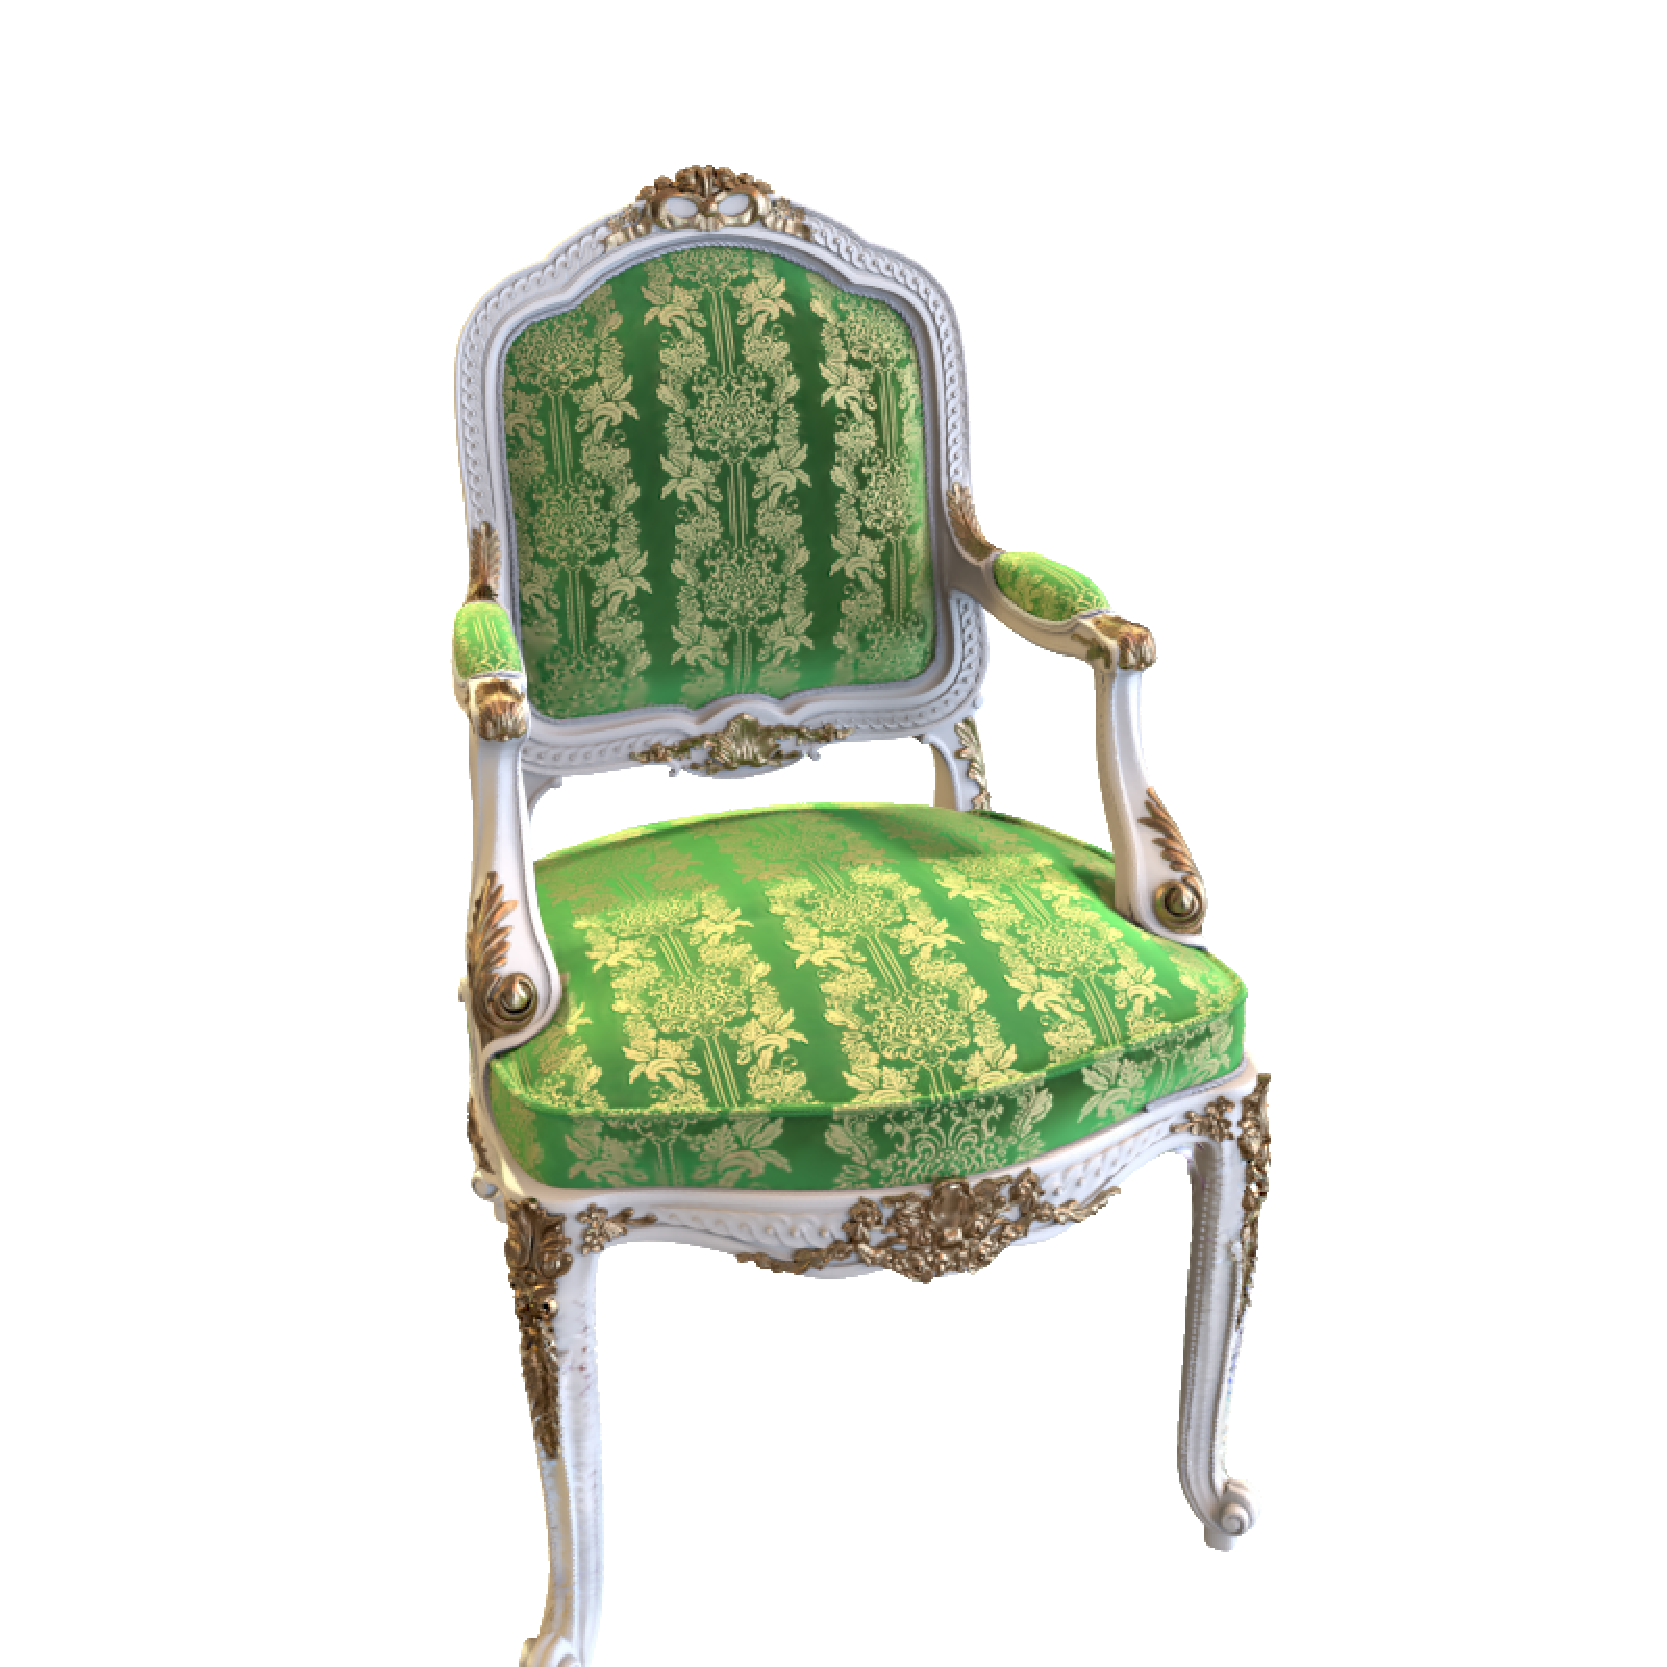
\includegraphics[width=0.19\linewidth]{./img/edit/geo/chair/00145}}&
            \hspace{-3mm}{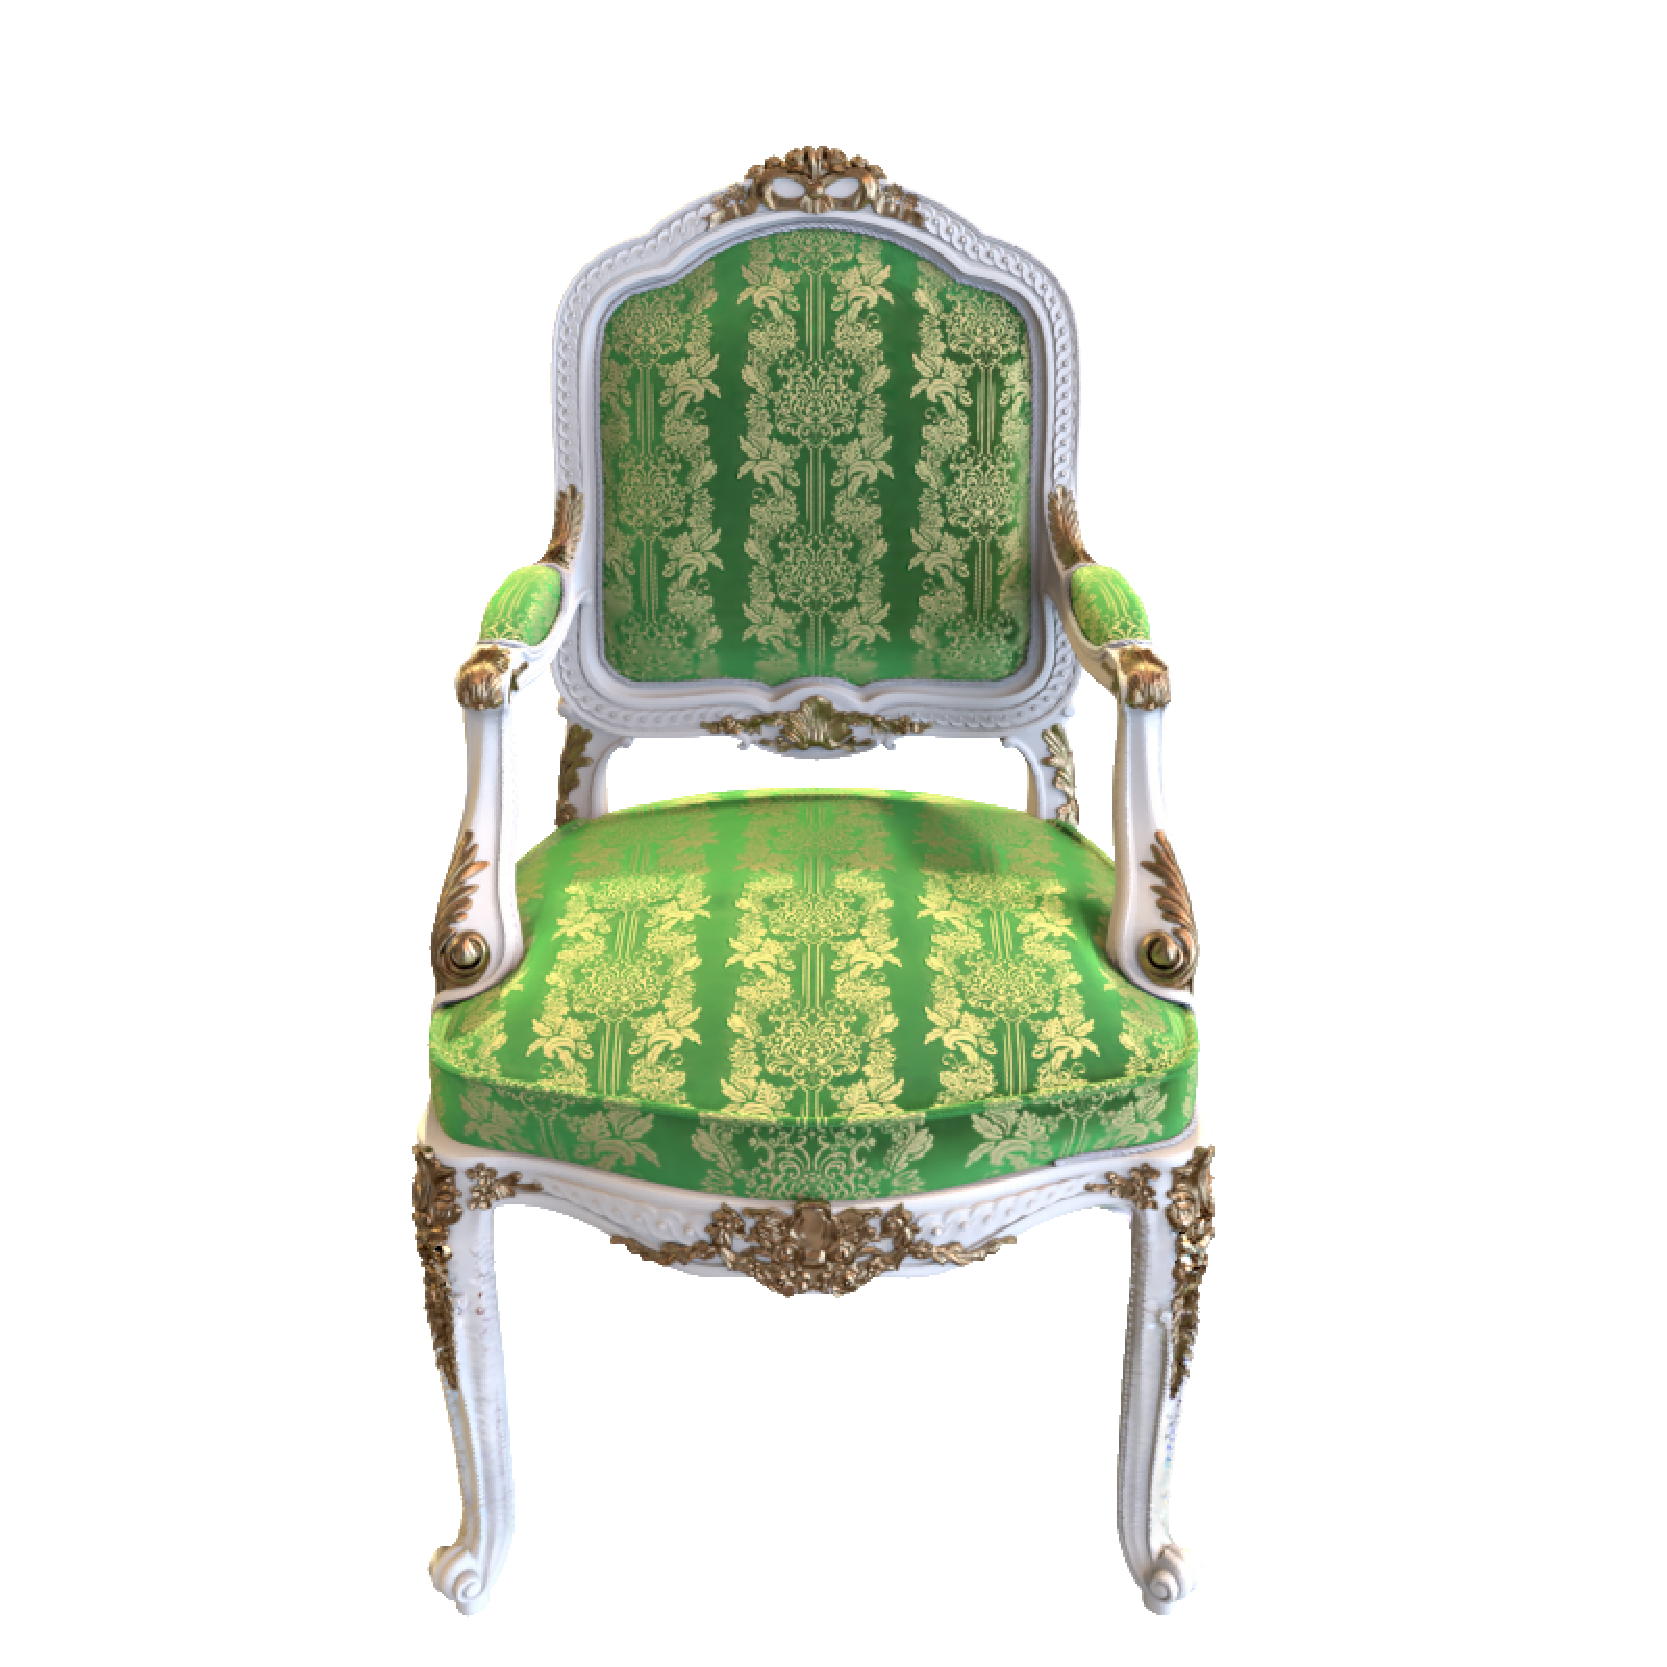
\includegraphics[width=0.19\linewidth]{./img/edit/geo/chair/00150}}&
            \hspace{-3mm}{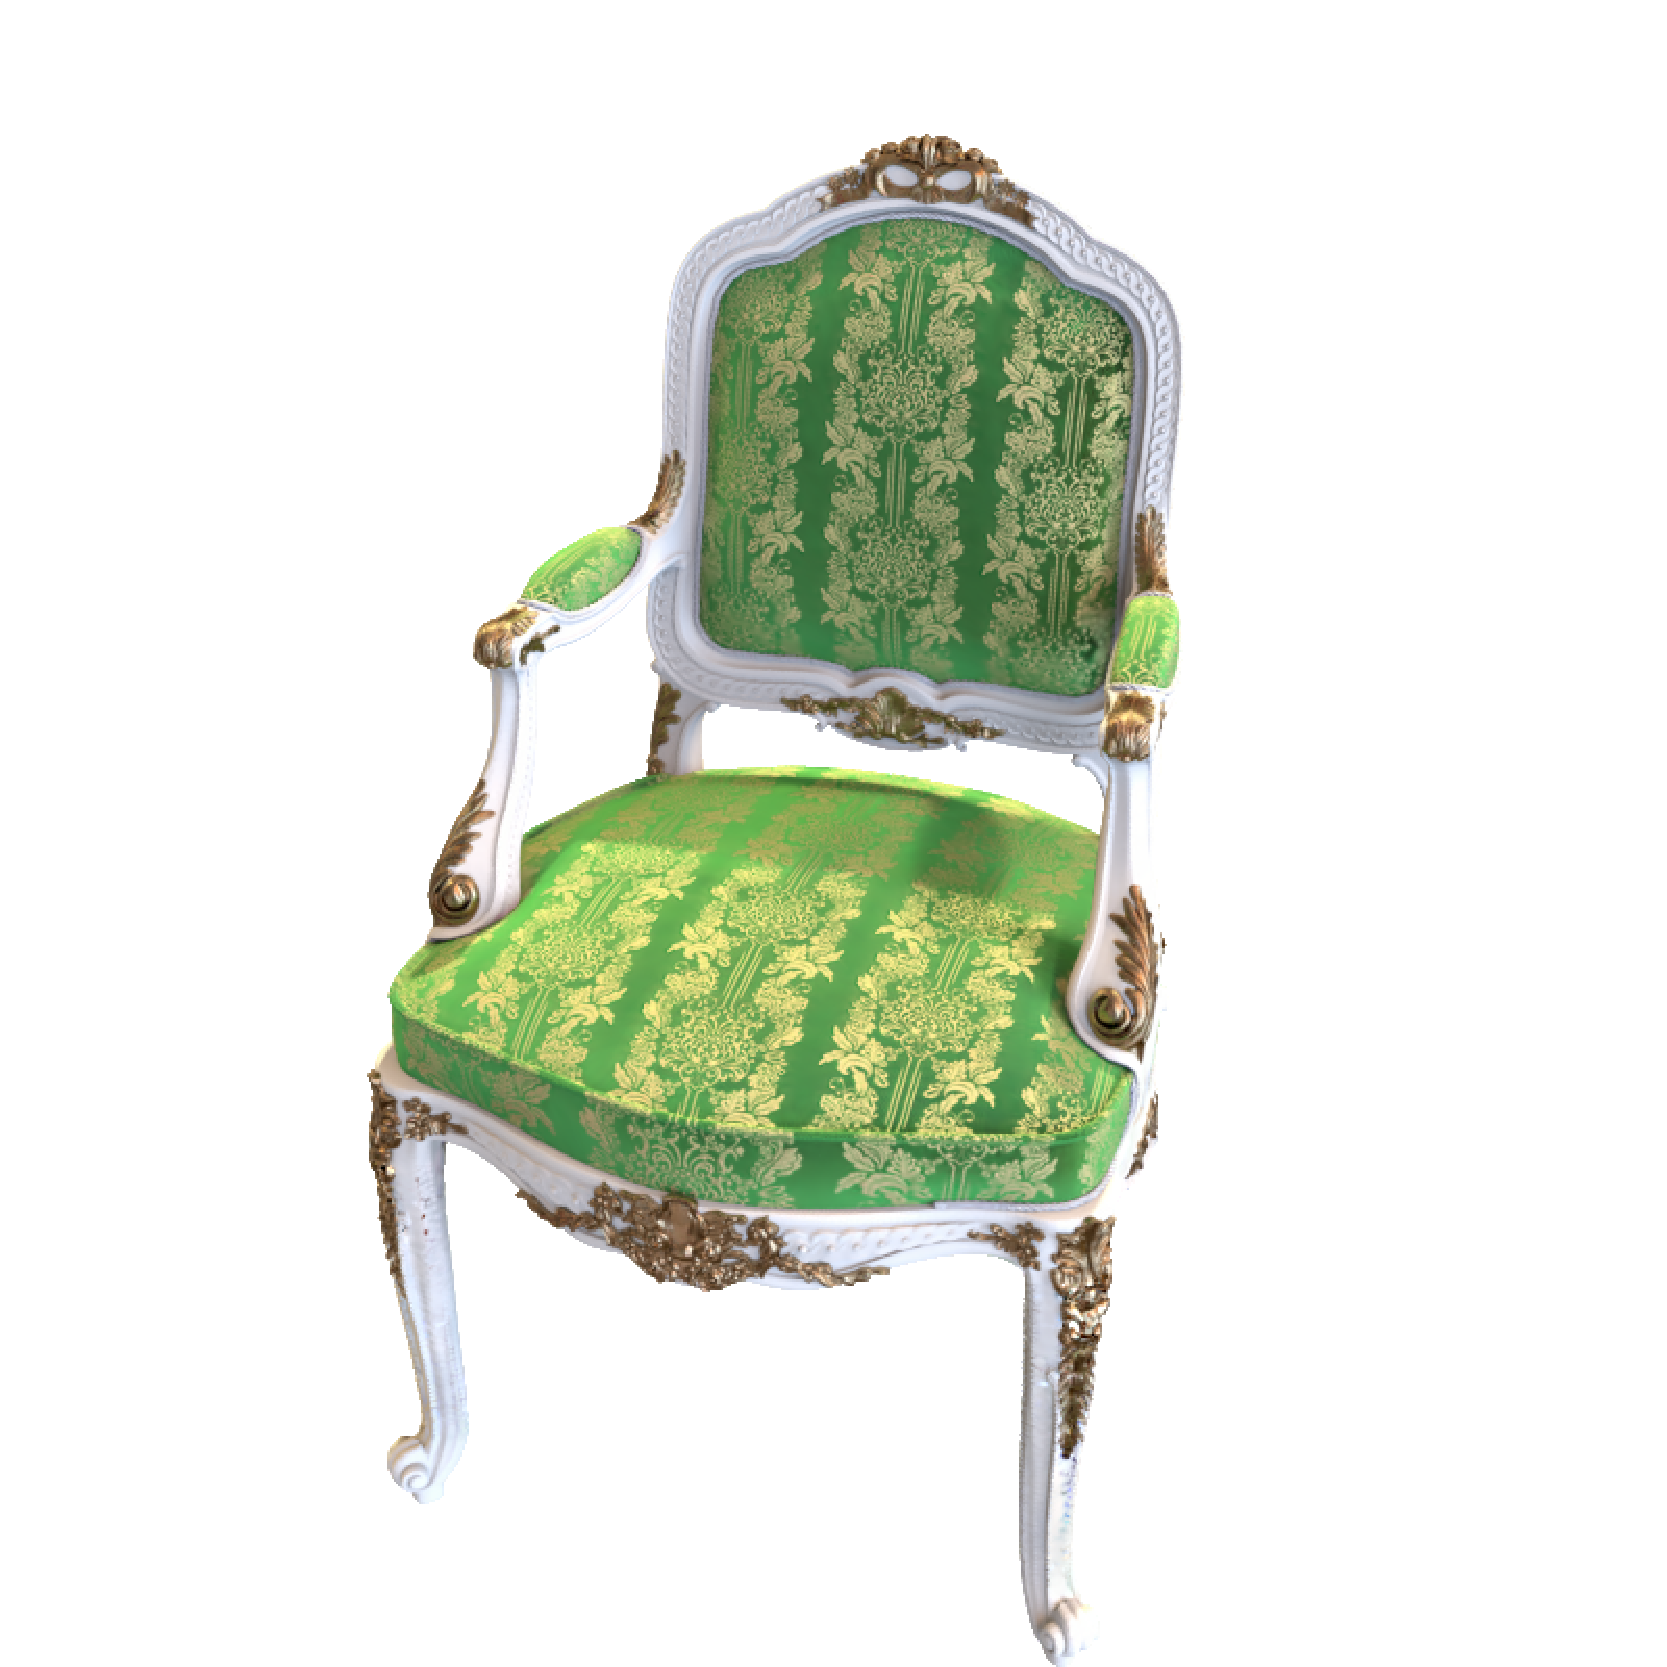
\includegraphics[width=0.19\linewidth]{./img/edit/geo/chair/00155}}
            \\
            \hspace{-4mm}
            \rotatebox{90}{\quad \hspace{-3mm} {\small Geometry}}
            &
            \hspace{-3mm}{
\includegraphics[width=0.19\linewidth]{./img/edit/geo/mic/input}}&
            \hspace{-3mm}{
\includegraphics[width=0.19\linewidth]{./img/edit/geo/mic/edit}}&
            \hspace{-3mm}{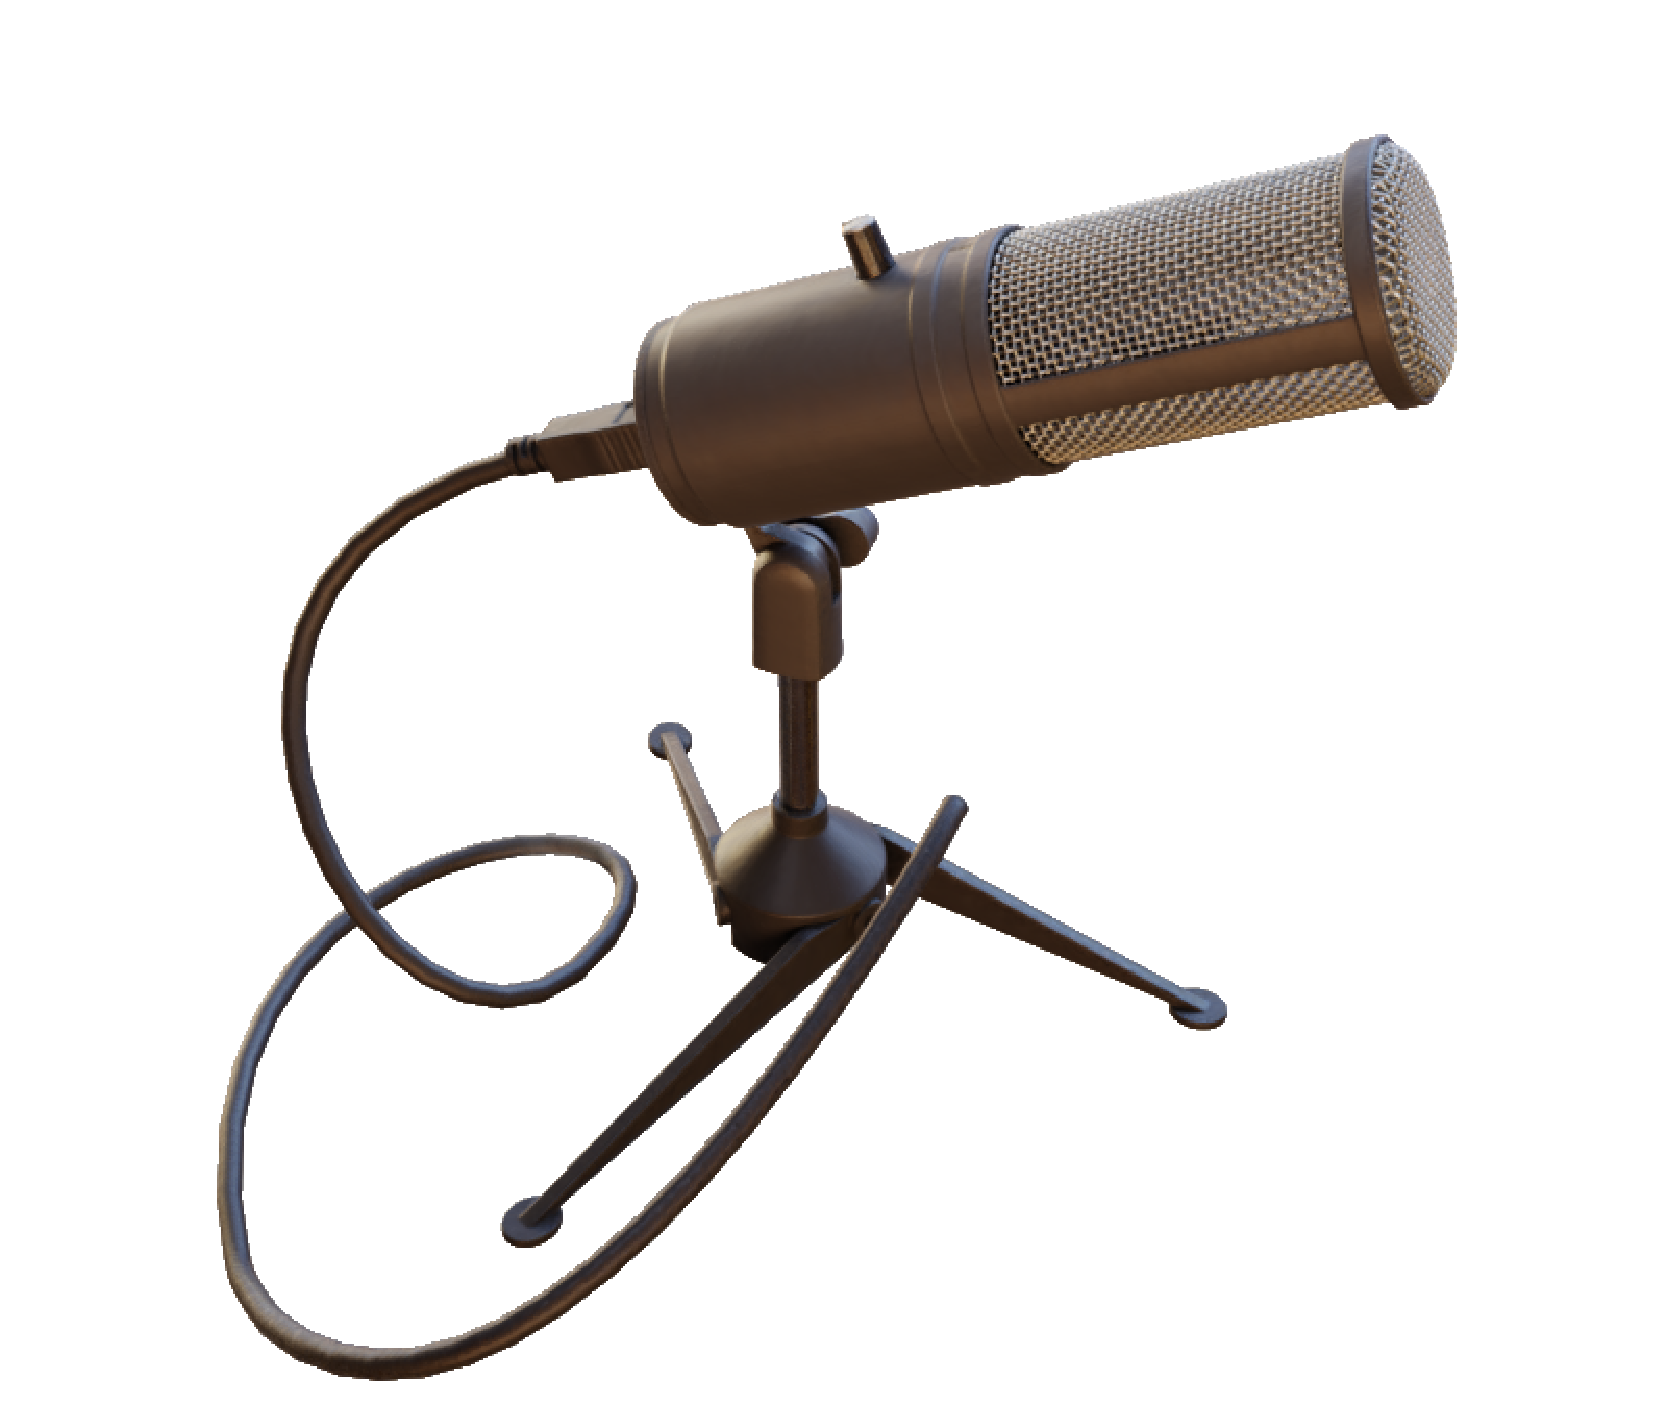
\includegraphics[width=0.19\linewidth]{./img/edit/geo/mic/00030}}&
            \hspace{-3mm}{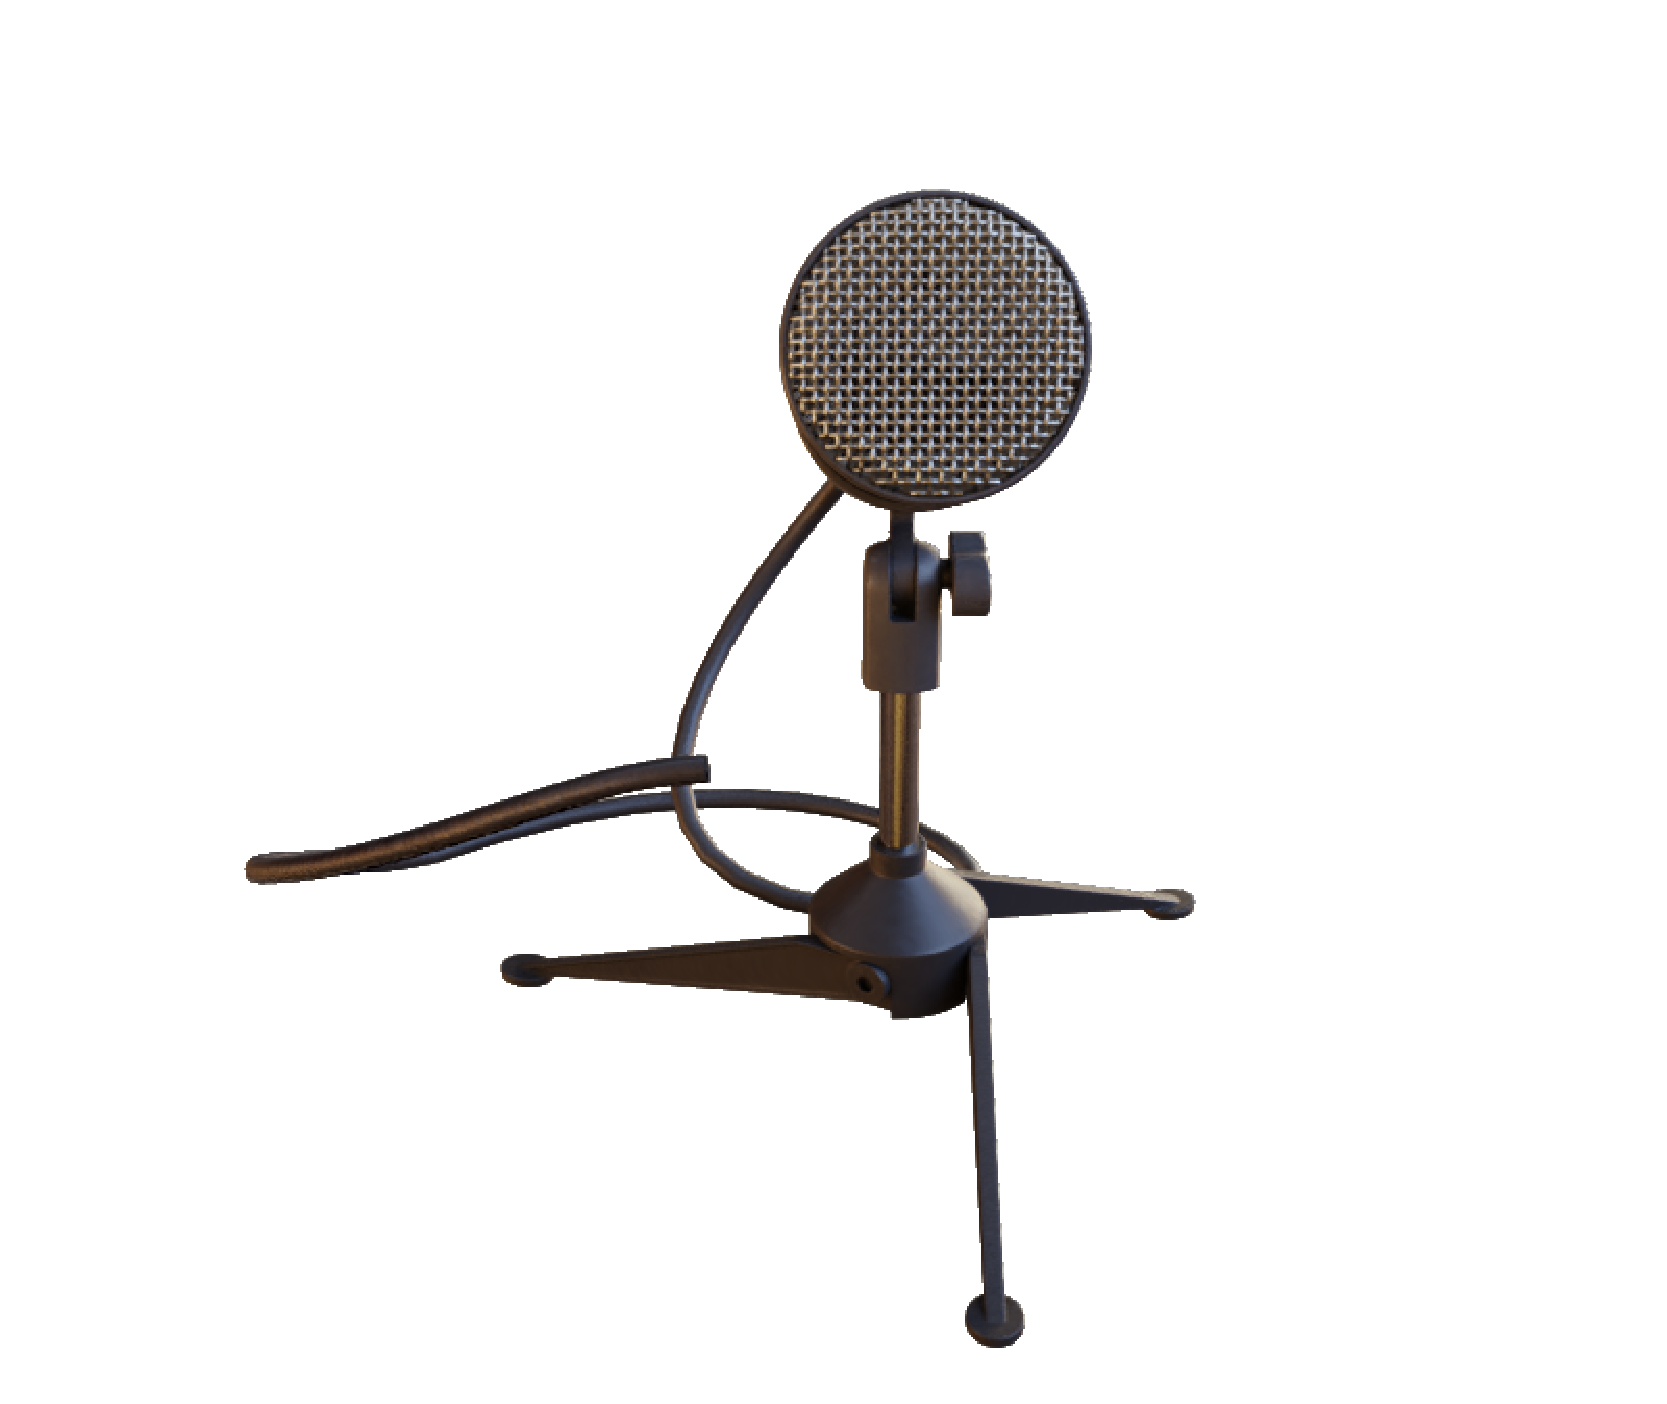
\includegraphics[width=0.19\linewidth]{./img/edit/geo/mic/00050}}&
            \hspace{-3mm}{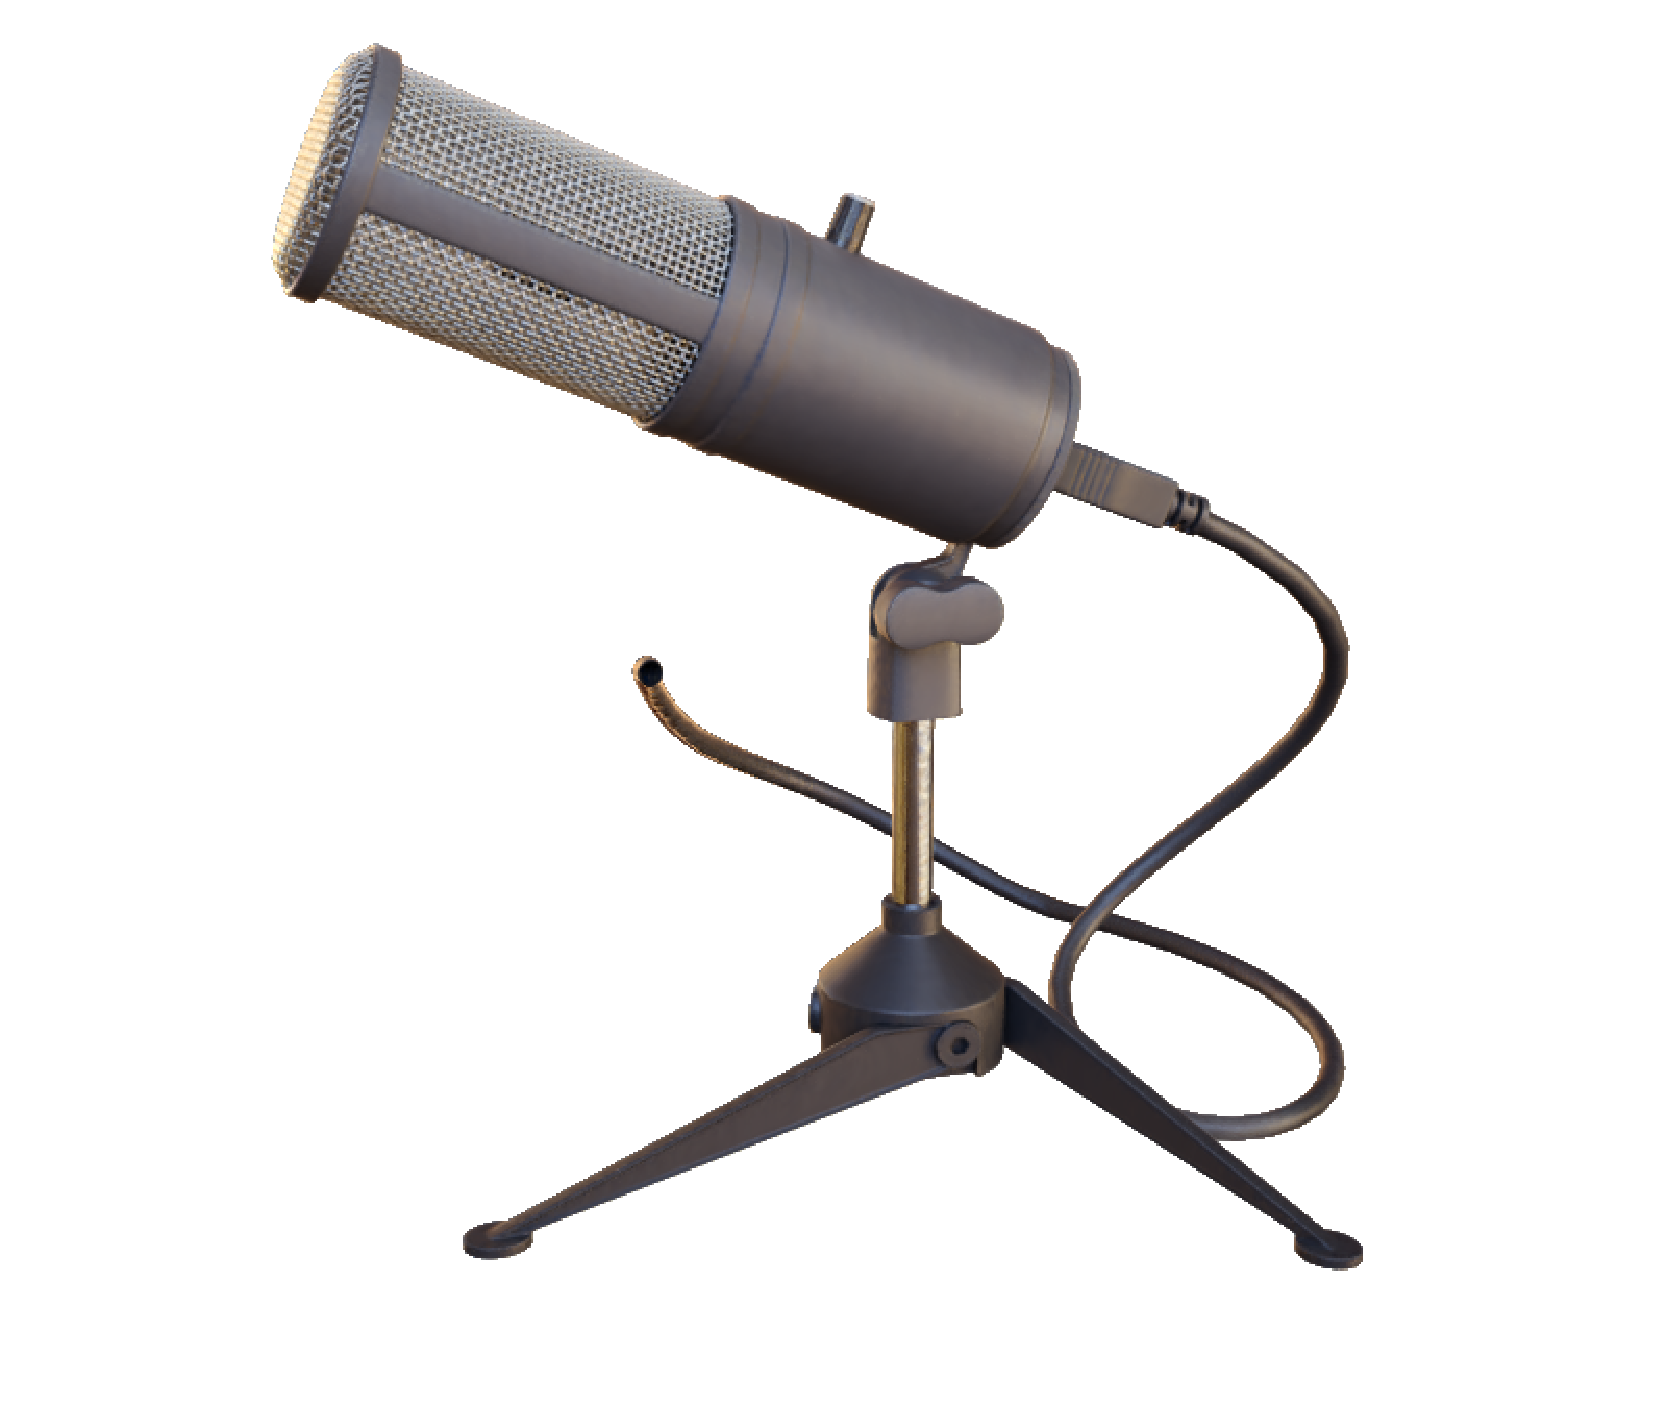
\includegraphics[width=0.19\linewidth]{./img/edit/geo/mic/00070}}
            \\
            \hspace{-4mm}
            \rotatebox{90}{\quad \hspace{-1mm} {\small Texture}}
            &
            \hspace{-3mm}{
\includegraphics[width=0.19\linewidth]{./img/edit/texture/car_siggraph_logo/input}}&
            \hspace{-3mm}{
\includegraphics[width=0.19\linewidth]{./img/edit/texture/car_siggraph_logo/edit}}&
            \hspace{-3mm}{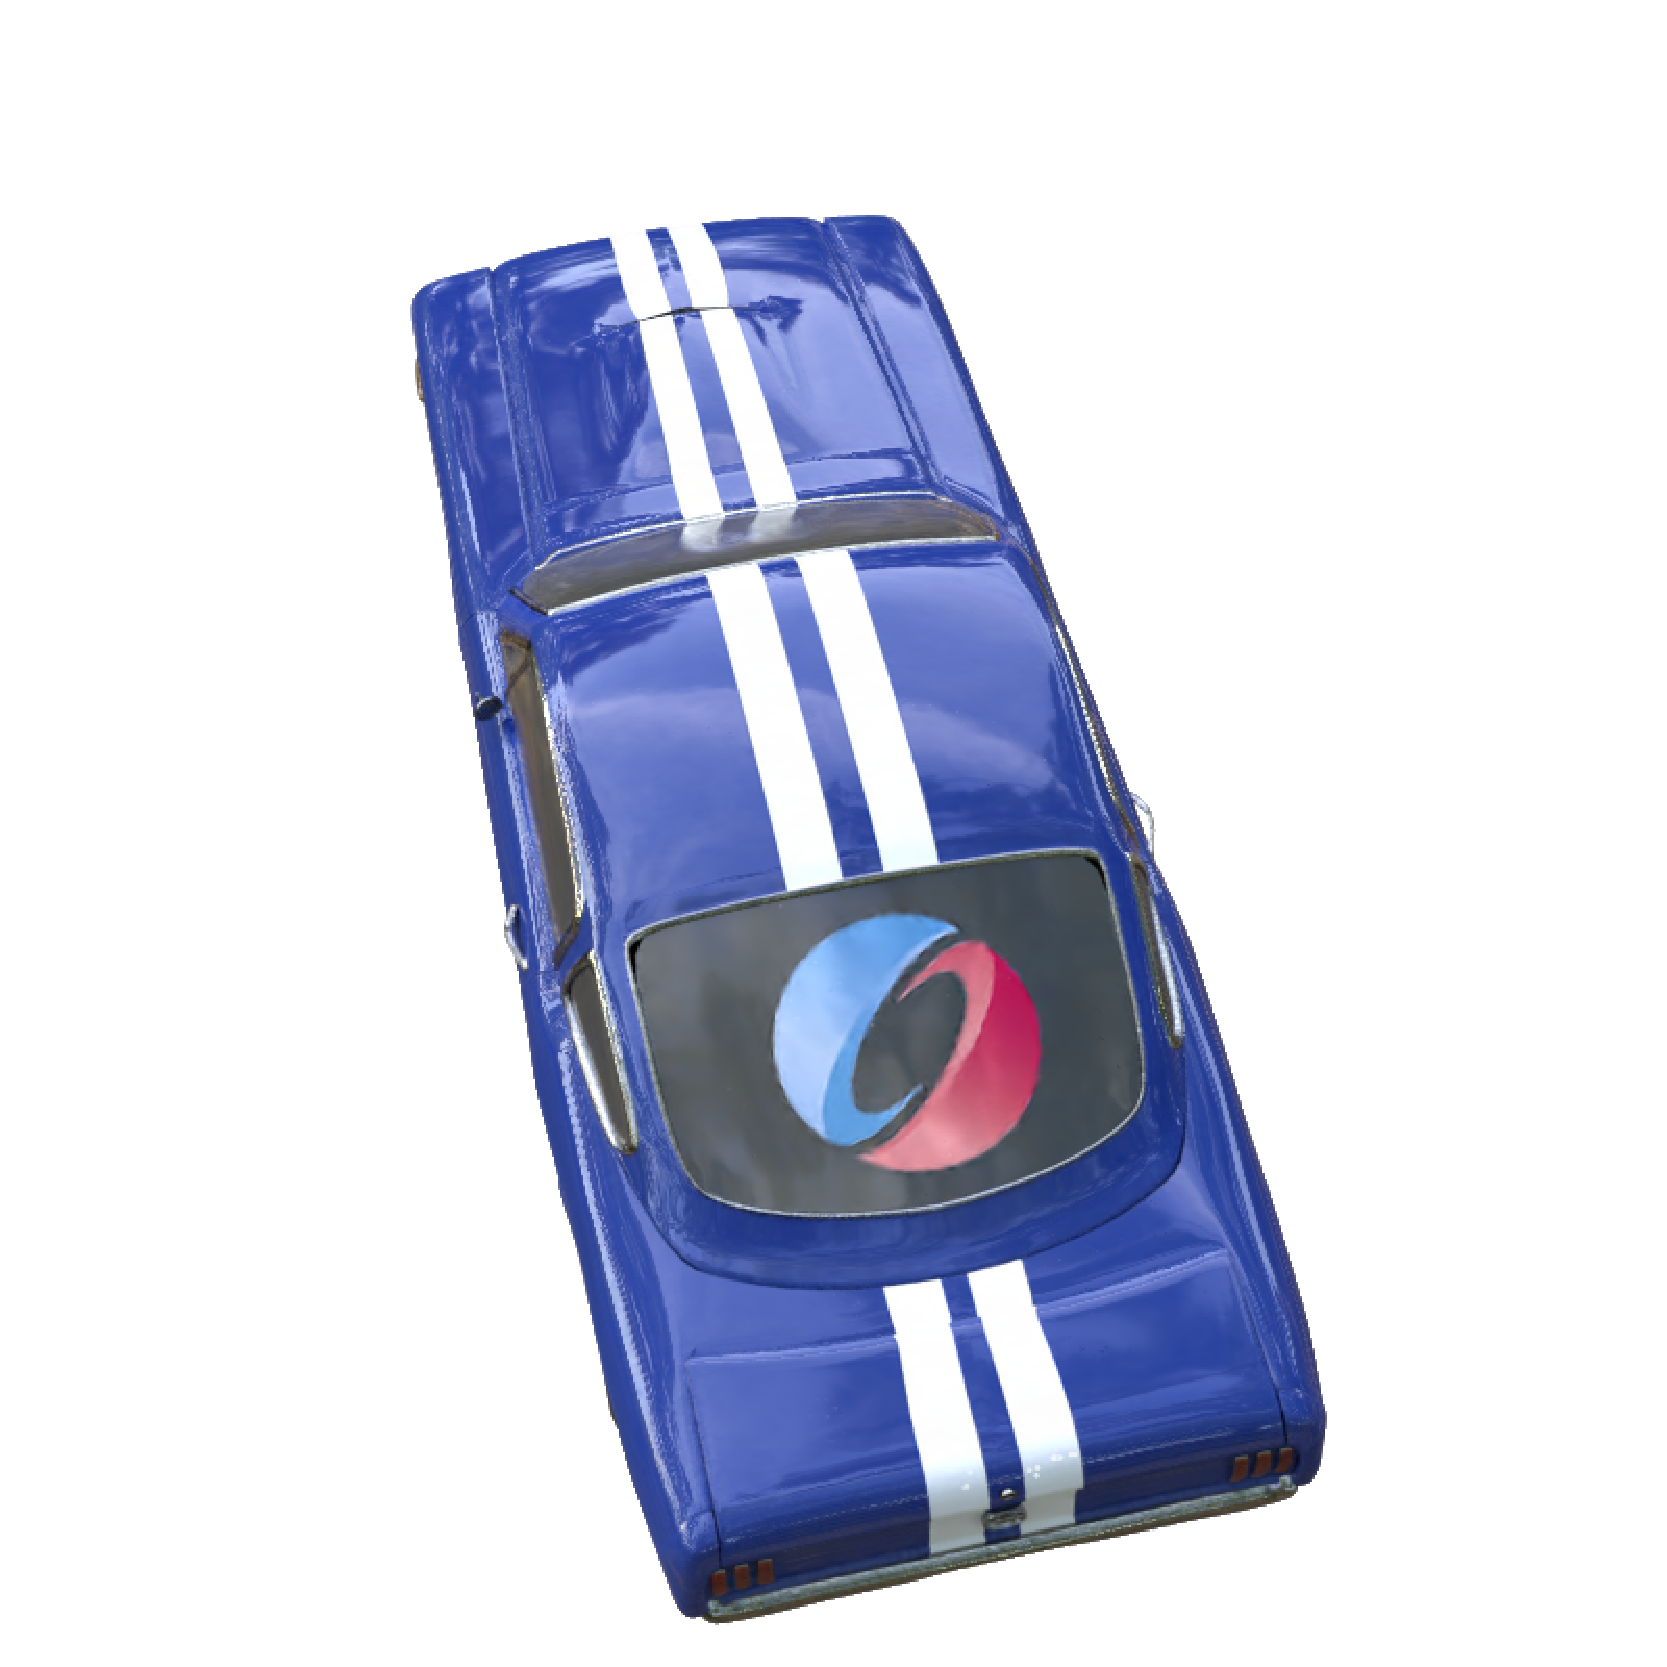
\includegraphics[width=0.19\linewidth]{./img/edit/texture/car_siggraph_logo/00011}}&
            \hspace{-3mm}{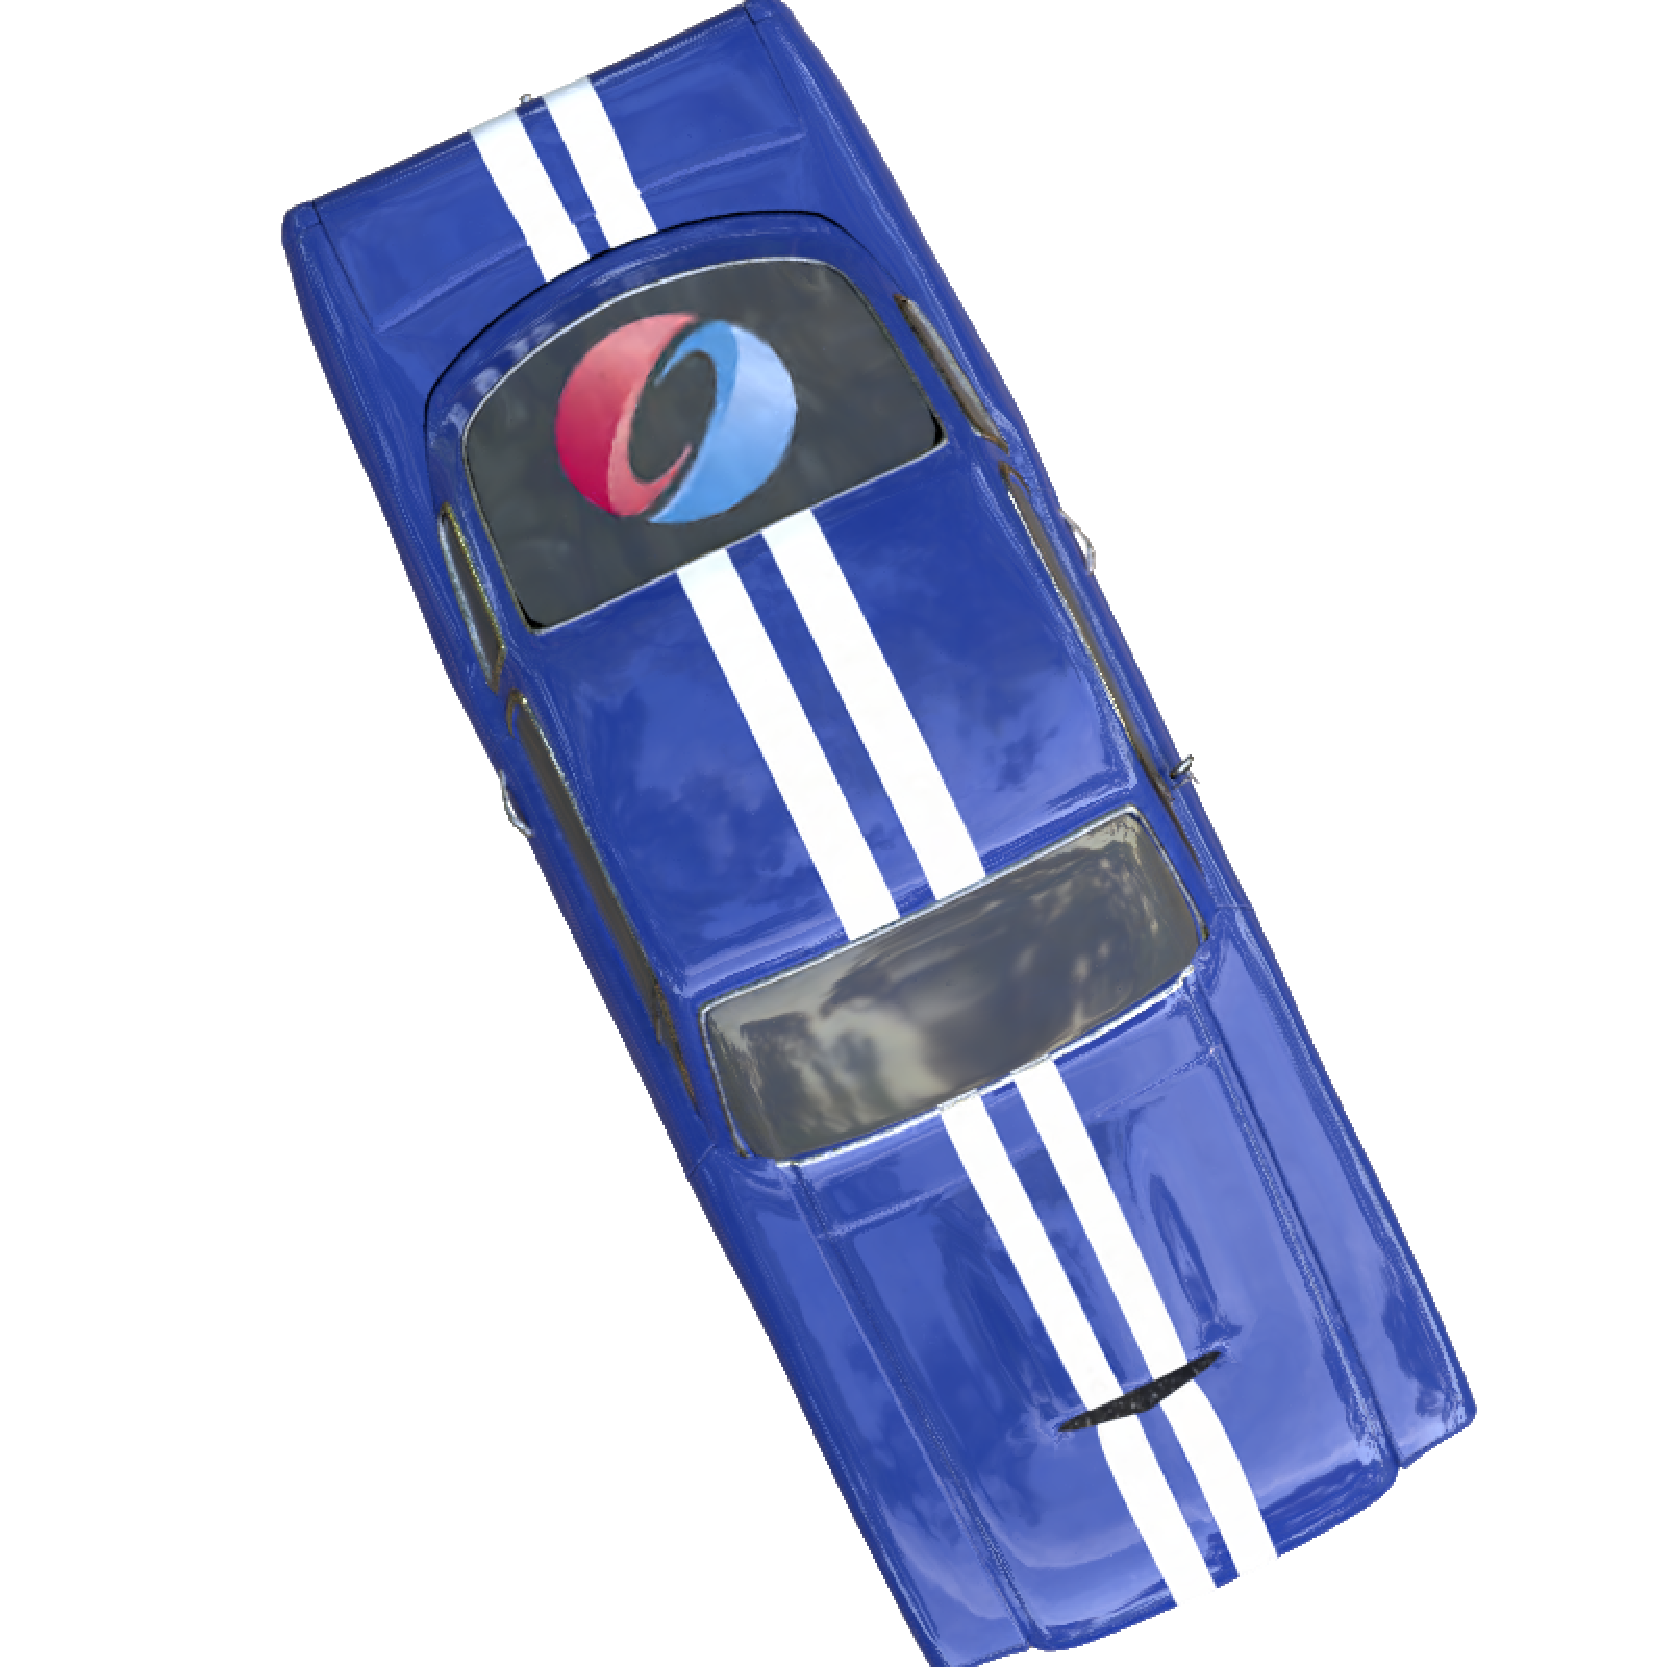
\includegraphics[width=0.19\linewidth]{./img/edit/texture/car_siggraph_logo/00007}}&
            \hspace{-3mm}{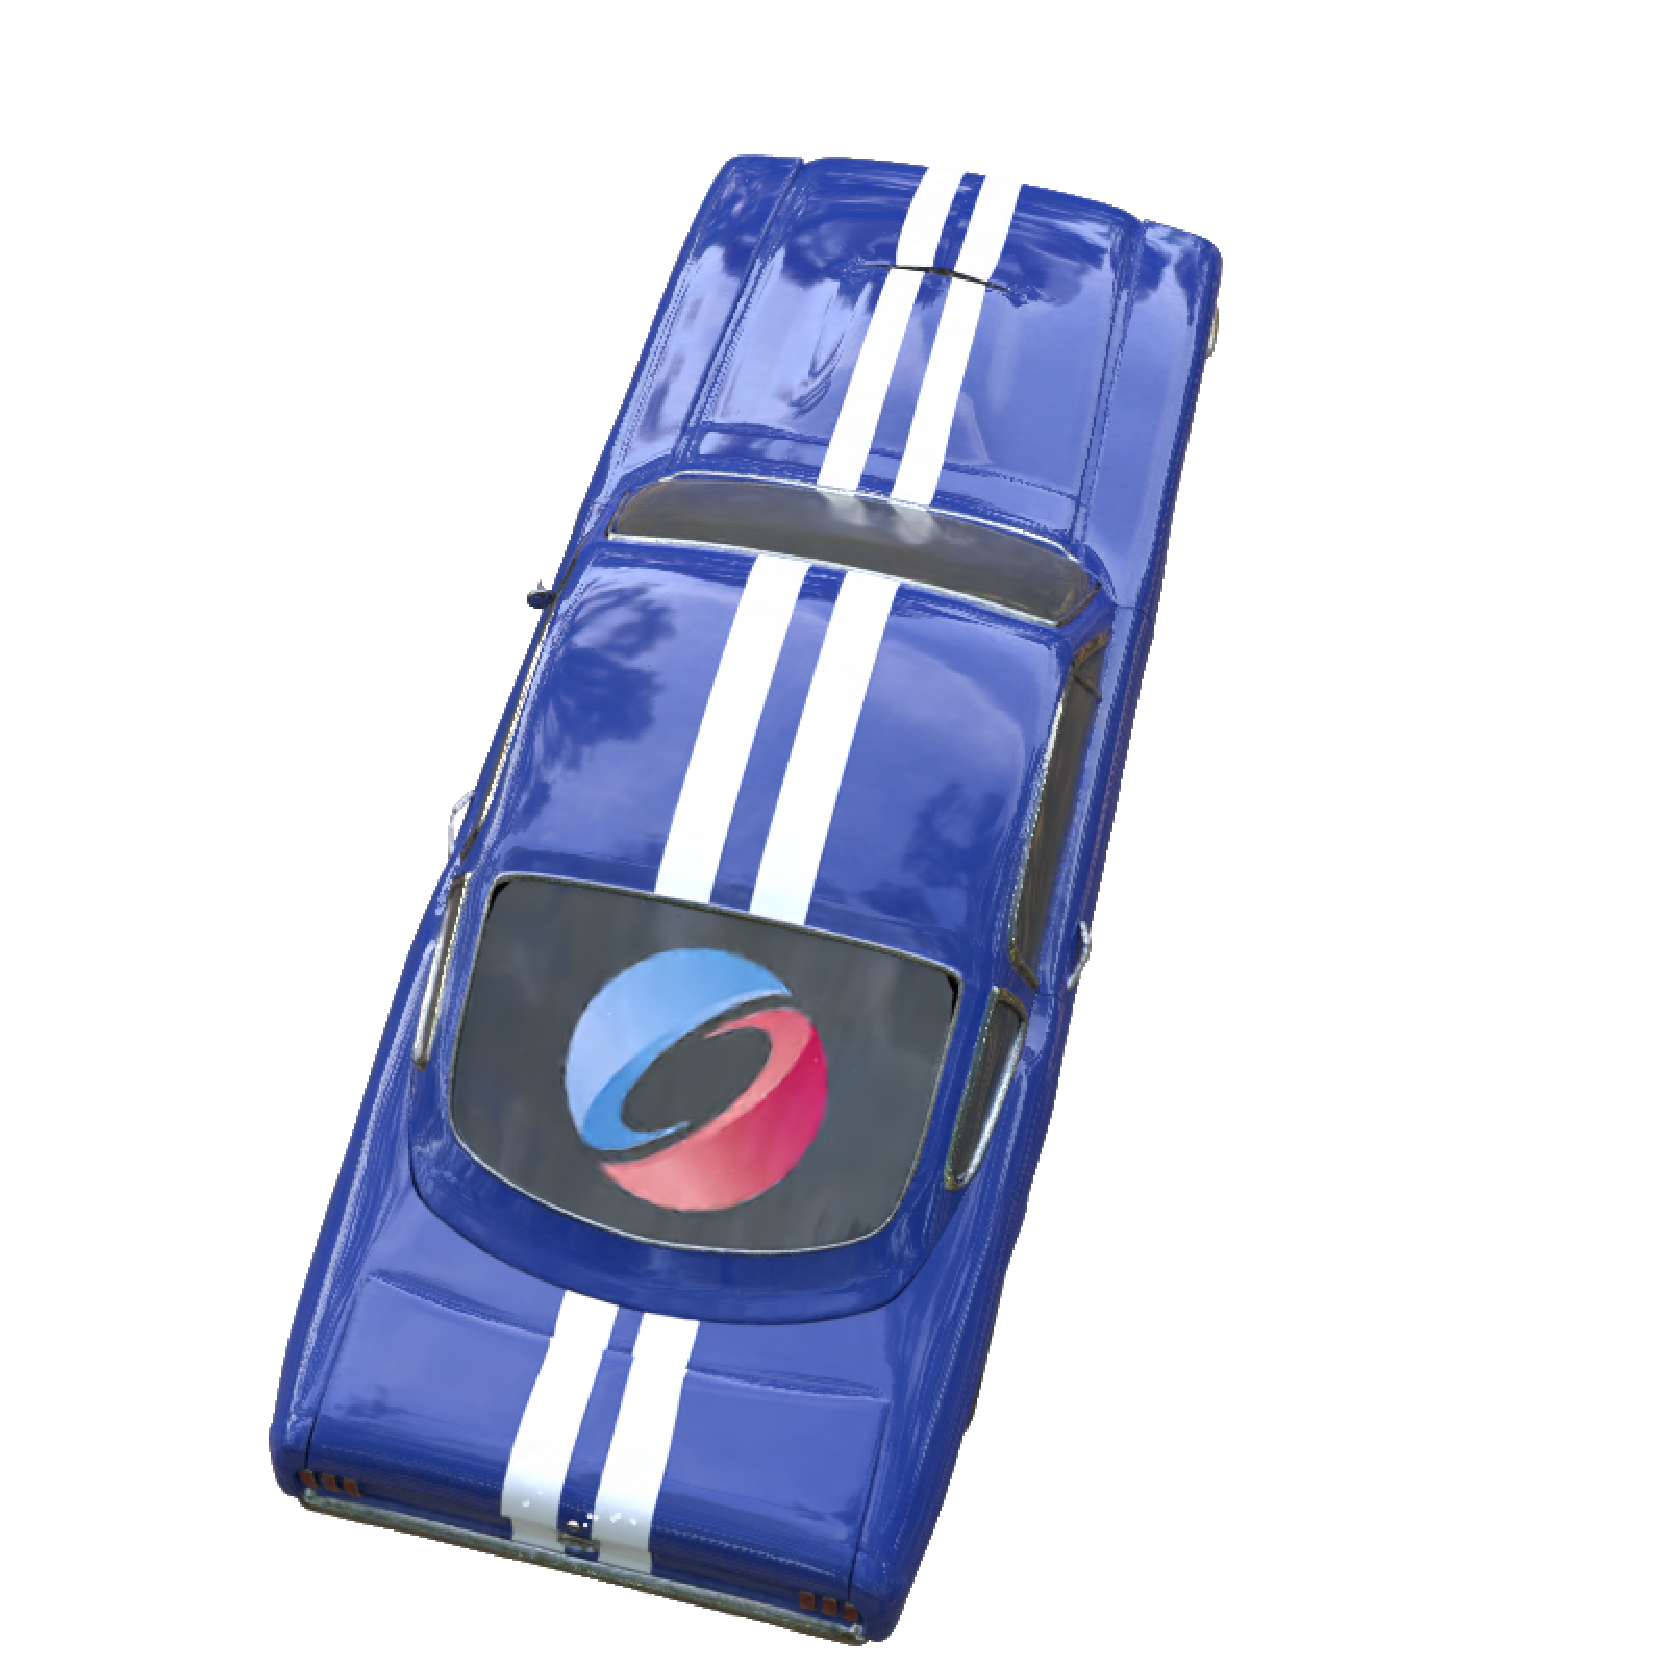
\includegraphics[width=0.19\linewidth]{./img/edit/texture/car_siggraph_logo/00012}}
            \\
            \hspace{-4mm}
            \rotatebox{90}{\quad \hspace{-2mm} {\small Texture}}
            &
            \hspace{-3mm}{
\includegraphics[width=0.19\linewidth]{./img/edit/texture/hotdog/input}}&
            \hspace{-3mm}{
\includegraphics[width=0.19\linewidth]{./img/edit/texture/hotdog/edit}}&
            \hspace{-3mm}{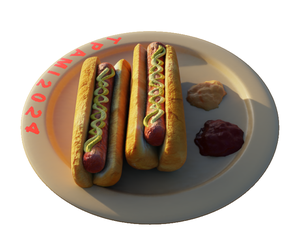
\includegraphics[width=0.19\linewidth]{./img/edit/texture/hotdog/0}}&
            \hspace{-3mm}{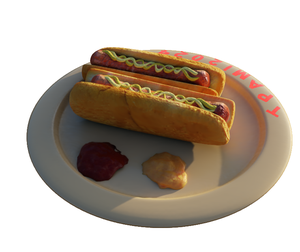
\includegraphics[width=0.19\linewidth]{./img/edit/texture/hotdog/30}}&
            \hspace{-3mm}{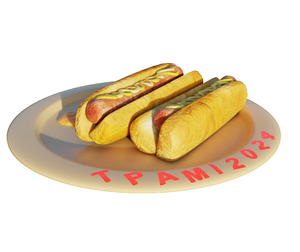
\includegraphics[width=0.19\linewidth]{./img/edit/texture/hotdog/60}}
            \\
            \hspace{-4mm}
            \rotatebox{90}{\quad \hspace{-2mm} {\small Texture}}
            &
            \hspace{-3mm}{
\includegraphics[width=0.19\linewidth]{./img/edit/texture/curry_scene001/input}}&
            \hspace{-3mm}{
\includegraphics[width=0.19\linewidth]{./img/edit/texture/curry_scene001/edit}}&
            \hspace{-3mm}{
\includegraphics[width=0.19\linewidth]{./img/edit/texture/curry_scene001/0004}}&
            \hspace{-3mm}{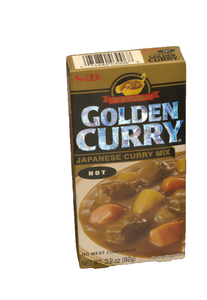
\includegraphics[width=0.19\linewidth]{./img/edit/texture/curry_scene001/0049}}&
            \hspace{-3mm}{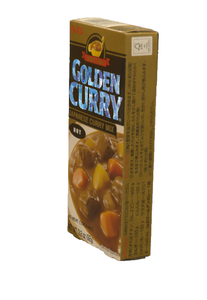
\includegraphics[width=0.19\linewidth]{./img/edit/texture/curry_scene001/0015}}
            \\
            &
            \hspace{-4mm}\makecell{Input}&
            \hspace{-4mm}\makecell{Edit}&
            \hspace{-4mm}\makecell{View \#1}&
            \hspace{-4mm}\makecell{View \#2}&
            \hspace{-4mm}\makecell{View \#3}
        \end{tabular}
    }
    \caption{
        Geometry editing and texture editing results. 
        For each row, we show input and edited geometry/image in the first two columns, and in the \yl{remaining} three columns we show edited \yl{Gaussians} rendered from three different viewpoints. 
    }
    \label{fig:geo_texture_edit}
\end{figure}


\subsection{Ablation}
In this subsection, we conduct several ablation studies to prove the effectiveness of our design choices. 

\subsection{Normal Field Distillation}
To produce a plausible geometry for the decomposition problem, we distill the normal direction from a signed distance function by encouraging the rendered normal of \yl{Gaussians} to be consistent with the normal of a signed distance function. 
Here, we generate the decomposed results without normal field distillation (w/o NFD) and compare them with the full pipeline qualitatively in Fig.~\ref{fig:ablate_NFD}. 
We also report numerical results of decomposed results in Table~\ref{tab:decom} and the decomposition quality sees a drop without normal field distillation. 
\begin{figure}[t]
        \centering
        {
            \begin{tabular}{ccc}
                \hspace{-2mm}
                {
\includegraphics[width=0.19\linewidth]{./img/ablate_nfd/materials/input}}
                {
\includegraphics[width=0.19\linewidth]{./img/ablate_nfd/materials/wo_n}}
                {
\includegraphics[width=0.19\linewidth]{./img/ablate_nfd/materials/w_n}}
                {
\includegraphics[width=0.19\linewidth]{./img/ablate_nfd/materials/wo_a}}
                {
\includegraphics[width=0.19\linewidth]{./img/ablate_nfd/materials/w_a}}
                \\
                \hspace{-2mm}
                \subcaptionbox{\scriptsize Input}{
\includegraphics[width=0.19\linewidth]{./img/ablate_nfd/ficus/input}}
                \subcaptionbox{\scriptsize w/o NFD}{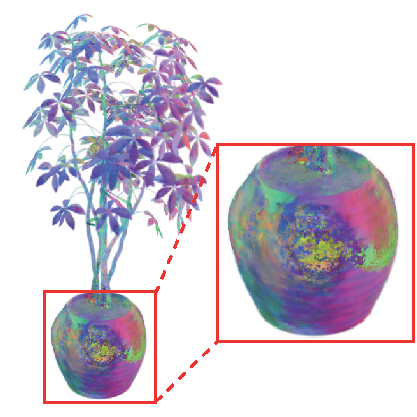
\includegraphics[width=0.19\linewidth]{./img/ablate_nfd/ficus/wo_n}}
                \subcaptionbox{\scriptsize w/ NFD}{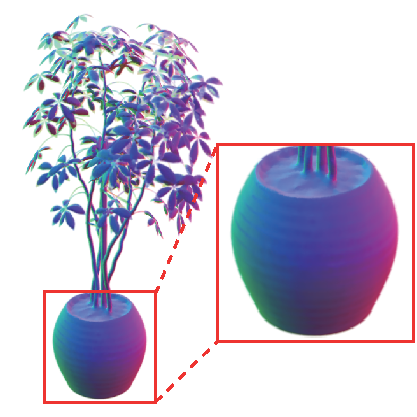
\includegraphics[width=0.19\linewidth]{./img/ablate_nfd/ficus/w_n}}
                \subcaptionbox{\scriptsize w/o NFD}{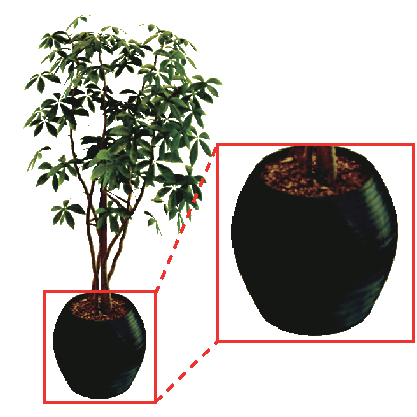
\includegraphics[width=0.19\linewidth]{./img/ablate_nfd/ficus/wo_a}}
                \subcaptionbox{\scriptsize w/ NFD}{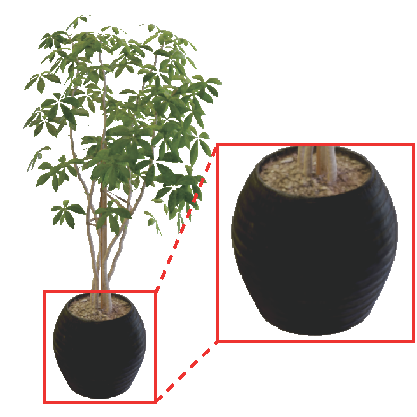
\includegraphics[width=0.19\linewidth]{./img/ablate_nfd/ficus/w_a}}
            \end{tabular}
        }
        \caption{
            Qualitative comparisons between decomposed normals and diffuse albedos with normal field distillation (w/ NFD) and without normal field distillation (w/o NFD). 
        }
        \label{fig:ablate_NFD}
\end{figure}


\subsection{Deferred Shading}
In the decomposition and relighting process, we utilize the \textit{deferred shading} technique instead \yl{of} \textit{forward shading} commonly used in previous methods. 
Here we ablate its influence on the relighting results in Fig.~\ref{fig:ablate_DS}. 
\wttp{Even \yl{though} the geometry is enhanced by the normal field distillation, we can \yl{still} observe notable Gaussian shape---like blending artifacts when we apply the \textit{forward shading} technique.} 
By contrast, the \textit{deferred shading} technique we use can successfully resolve this issue and produce smooth and realistic relighting results. 
We also evaluate it quantitatively in Table~\ref{tab:relight} and the relighting quality drops when it is not applied. 

\begin{figure}[t]
    \centering
    {
        \begin{tabular}{c}
            \hspace{-4mm}
            {
\includegraphics[width=0.16\linewidth]{./img/ablate_ds/toaster/forest/input}}
            {
\includegraphics[width=0.16\linewidth]{./img/ablate_ds/toaster/forest/fs}}
            {
\includegraphics[width=0.16\linewidth]{./img/ablate_ds/toaster/forest/ds}}
            {
\includegraphics[width=0.16\linewidth]{./img/ablate_ds/toaster/sunset/input}}
            {
\includegraphics[width=0.16\linewidth]{./img/ablate_ds/toaster/sunset/fs}}
            {
\includegraphics[width=0.16\linewidth]{./img/ablate_ds/toaster/sunset/ds}}
            \\
            \hspace{-4mm}
            {
\includegraphics[width=0.16\linewidth]{./img/ablate_ds/helmet/forest/input}}
            {
\includegraphics[width=0.16\linewidth]{./img/ablate_ds/helmet/forest/fs}}
            {
\includegraphics[width=0.16\linewidth]{./img/ablate_ds/helmet/forest/ds}}
            {
\includegraphics[width=0.16\linewidth]{./img/ablate_ds/helmet/sunset/input}}
            {
\includegraphics[width=0.16\linewidth]{./img/ablate_ds/helmet/sunset/fs}}
            {
\includegraphics[width=0.16\linewidth]{./img/ablate_ds/helmet/sunset/ds}}
            \\
            \hspace{-4mm}
            {
\includegraphics[width=0.16\linewidth]{./img/ablate_ds/pitcher_scene001/pitcher_scene005_0068/input}}
            {
\includegraphics[width=0.16\linewidth]{./img/ablate_ds/pitcher_scene001/pitcher_scene005_0068/fs}}
            {
\includegraphics[width=0.16\linewidth]{./img/ablate_ds/pitcher_scene001/pitcher_scene005_0068/ds}}
            {
\includegraphics[width=0.16\linewidth]{./img/ablate_ds/pitcher_scene001/pitcher_scene007_0065/input}}
            {
\includegraphics[width=0.16\linewidth]{./img/ablate_ds/pitcher_scene001/pitcher_scene007_0065/fs}}
            {
\includegraphics[width=0.16\linewidth]{./img/ablate_ds/pitcher_scene001/pitcher_scene007_0065/ds}}
            \\
            \hspace{-4mm}
            \subcaptionbox{Input}{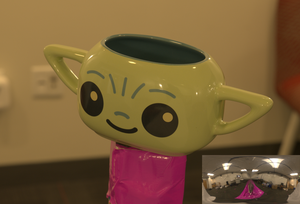
\includegraphics[width=0.16\linewidth]{./img/ablate_ds/grogu_scene001/grogu_scene001_0000/input}}
            \subcaptionbox{F.S.}{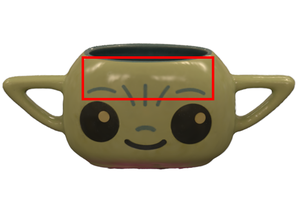
\includegraphics[width=0.16\linewidth]{./img/ablate_ds/grogu_scene001/grogu_scene001_0000/fs}}
            \subcaptionbox{D.S.}{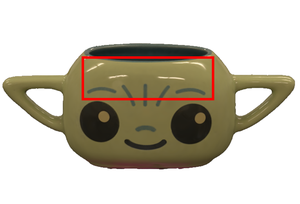
\includegraphics[width=0.16\linewidth]{./img/ablate_ds/grogu_scene001/grogu_scene001_0000/ds}}
            \subcaptionbox{Input}{
\includegraphics[width=0.16\linewidth]{./img/ablate_ds/grogu_scene001/studio/input}}
            \subcaptionbox{F.S.}{
\includegraphics[width=0.16\linewidth]{./img/ablate_ds/grogu_scene001/studio/fs}}
            \subcaptionbox{D.S.}{
\includegraphics[width=0.16\linewidth]{./img/ablate_ds/grogu_scene001/studio/ds}}
        \end{tabular}
    }
    \caption{
        Qualitative comparisons between relighting results with \textit{forward shading} (F.S.) and with \textit{deferred shading} (D.S.). 
        The relit scene contains blending artifacts when we use \textit{forward shading} while \textit{deferred shading} can avoid them. 
        The bottom two rows are from the real Stanford ORB dataset~\cite{Stanford-ORB}.
    }
     \vspace{-3mm}
    \label{fig:ablate_DS}
\end{figure}

\begin{figure}[!h]
    \centering
    {
        \begin{tabular}{c}
            \hspace{-4mm}
            {
\includegraphics[width=0.16\linewidth]{./img/ablate_texture_edit/toaster/input}}
            {
\includegraphics[width=0.16\linewidth]{./img/ablate_texture_edit/toaster/edit}}
            {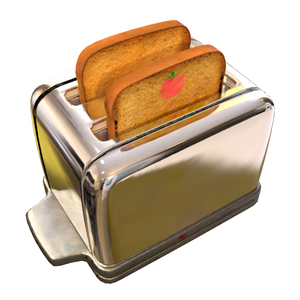
\includegraphics[width=0.16\linewidth]{./img/ablate_texture_edit/toaster/wo_00016}}
            {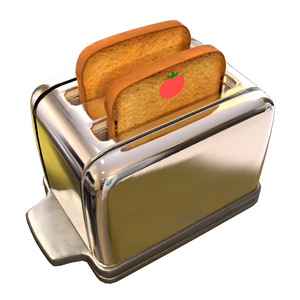
\includegraphics[width=0.16\linewidth]{./img/ablate_texture_edit/toaster/w_00016}}
            {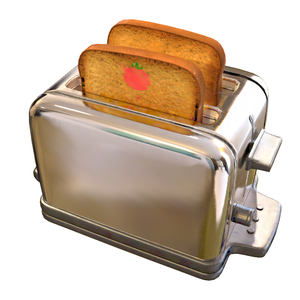
\includegraphics[width=0.16\linewidth]{./img/ablate_texture_edit/toaster/wo_00032}}
            {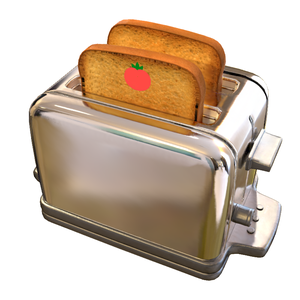
\includegraphics[width=0.16\linewidth]{./img/ablate_texture_edit/toaster/w_00032}}
            \\
            \hspace{-4mm}
            \subcaptionbox{\scriptsize Input}{
\includegraphics[width=0.16\linewidth]{./img/ablate_texture_edit/mic/input}}
            \subcaptionbox{\scriptsize Edit}{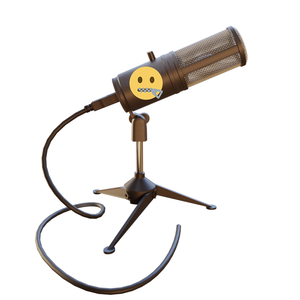
\includegraphics[width=0.16\linewidth]{./img/ablate_texture_edit/mic/edit}}
            \subcaptionbox{\scriptsize w/o R.V.}{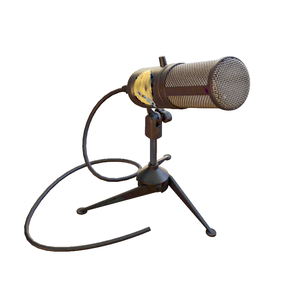
\includegraphics[width=0.16\linewidth]{./img/ablate_texture_edit/mic/wo_00040}}
            \subcaptionbox{\scriptsize w/ R.V.}{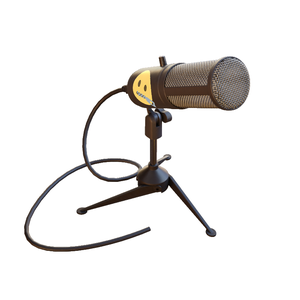
\includegraphics[width=0.16\linewidth]{./img/ablate_texture_edit/mic/w_00040}}
            \subcaptionbox{\scriptsize w/o R.V.}{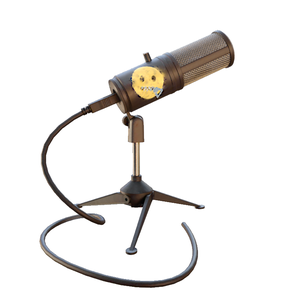
\includegraphics[width=0.16\linewidth]{./img/ablate_texture_edit/mic/wo_00120}}
            \subcaptionbox{\scriptsize w/ R.V.}{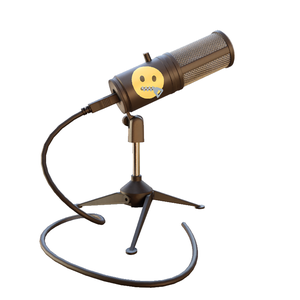
\includegraphics[width=0.16\linewidth]{./img/ablate_texture_edit/mic/w_00120}}
        \end{tabular}
    }
    \caption{
        \wttp{
        Qualitative comparisons between texture editing results with rendered results from random viewpoints (w/ R.V.) and without (w/o R.V.). 
        The rendered results of edited gaussians splatting from novel viewpoints can exhibit inconsistency without inputting rendered results from random viewpoints. 
        }
    }
    \label{fig:ablate_texture_edit}
\end{figure}


\wttp{
\subsection{Random View Inputs in Texture Editing}
As mentioned in Sec.~\ref{sec:texture_edit}, we perform texture editing on the Gaussian splatting representation by optimizing Gaussians' attributes to fit the rendered results to both the input edited image and randomly rendered images from different viewpoints. 
Here we ablate how randomly generated edited results influence the final rendered results of edited Gaussians in Fig.~\ref{fig:ablate_texture_edit}. 
It shows that optimizing Gaussians' attributes only from the input edited viewpoint can result in overfitting and exhibit inconsistent novel views. 
}

\begin{figure}[!h]
    \centering
    {
        \begin{tabular}{cc|cc}
            \hspace{-2mm}\subcaptionbox{\small Input}{
\includegraphics[width=0.24\linewidth]{./img/limit/decom/input.pdf}}&
            \hspace{-2mm}\subcaptionbox{\small Diffuse Albedo}{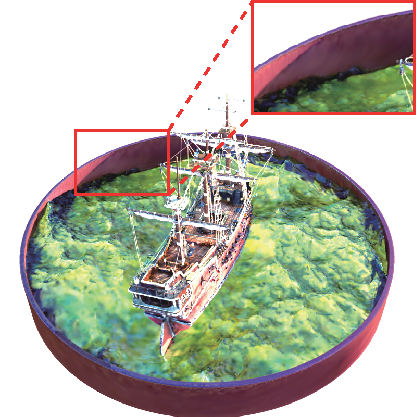
\includegraphics[width=0.24\linewidth]{./img/limit/decom/a.pdf}}&
            \hspace{-2mm}\subcaptionbox{\small Edit}{
\includegraphics[width=0.24\linewidth]{./img/limit/edit/edit.pdf}}&
            \hspace{-2mm}\subcaptionbox{\small Novel View}{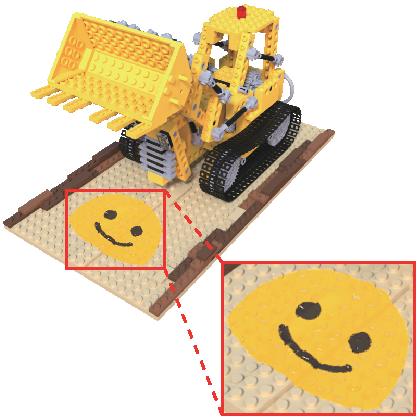
\includegraphics[width=0.24\linewidth]{./img/limit/edit/ours.pdf}}
        \end{tabular}
    }
    \caption{
        Limitations. \name bakes shadow into texture on scenes containing shadow ((a)-(b)) and may result in noises after texture editing ((c)-(d)).
    }
    \label{fig:limit}
\end{figure}


